\newpage
\chapter{Background Theory and Method}
% \addcontentsline{toc}{chapter}{Background Theory and Method} 

Small introtext to motivate this chapter. What am I going to go over here.




% The friction force is not an independent external force that acts on a body but an internal force that opposes the externally applied force. Thus, it may be thought of as a reaction force rather than an action force. In this sense, it is similar to the adhesion force between two bodies, which appears only when one tries to separate the bodies from contact. \cite{gao_frictional_2004}



% Read \cite{gao_frictional_2004} to fill in some gaps in the history below

\section{Tribology - friction}
Friction is a part of the wider field tribology which includes the study of
friction, wear and lubrication between two surfaces in relative motion \cite[p.
1]{gnecco_meyer_2015}. In this thesis we will only concern ourselves with so-called wearless dry friction. That is, without any use of lubrication and without any resulting wear of the contacting surfaces. Tribological systems take place across a broad
range of time and length scales, ranging from geological stratum layers involved
in earthquakes \cite{kim_nano-scale_2009} to microscopic atomistic processes, as
in the gliding motion of a nanocluster of a nanomotor \cite{Manini_2016}. This
vast difference in scale gives rises to different frictional mechanism being
dominating at different scales. On a macro scale the system is usally subject
to relatively high loads and speeds leading to high contact stresses and
wear. On the other hand, the micro-/nanoscale regime occupies the opposite domain operating under relatviely small loads and speeds with negligible wear \cite{kim_nano-scale_2009} \cite[p. 5]{bhushan_2013}. While macroscale friction is often reduced into a few variables such as load, material type, speed and surface roughness it is clear that the micro-/nanoscale friction cannot be generalized under such a simple representation. On the micro-/nanoscale the tribological propteries dominated by surface properties which will introduce an additional sensitivity variables such as temperature, humidity and even sliding history. The works of Bhushan and Kulkarni \cite[(1996)]{BHUSHAN199649} showed that the friction coefficient decreased with scale even though the materials used was unchanged. This reveals an intrinsic relationship between friction and scale as the contact condition is altered.

The phenomenological descriptions of macroscale friction cannot yet be derived from the fundamental atomic principles, and bridging the gap between different length scales in tribological systems remains an open challenge \cite{Manini_2016}. Hence, the following sections will be organized into macro-, micro- and nanoscale representing the theoretical understanding governing each scale regime. While our study of the graphene sheet is based on a nanoscale perspective the hypothesizing about application possibilities will eventually draw upon a macroscale perspective as well. Thus, we argue that a brief theoretical introduction to all three major scales is of high interest for a more complete interpreation of the findings in this thesis. 


% Tribological systems pose a wide range of dimensional scale. At the largest
% scale, geological stratum layers that are involved in earthquakes may be
% considered as a tribological system. The movement of the stratum occurs when
% the frictional forces between the layers are overcome by internal pressure
% inside the earth. At the smallest scale, relative motion of atoms at the
% interface of two materials would be a good example that involves frictional
% interaction. Owing to the vast difference in scale, the dominant mechanisms of
% friction and wear in macro-scale systems may be different from those of
% micro/nano-scale systems. In macro-scale, the tribological systems experience
% relatively large contact stresses and speeds. On the other hand,
% micro/nano-scale systems operate under relatively low loads and speeds.
% Particularly, the inertial effects that are prominent in macro-scale may be
% insignificant at the micro/nano-scale. Rather, surface forces often dictate
% the tribological interactions at small scales. \cite{kim_nano-scale_2009}.




% The differences between the conventional or macrotribology and
% micro/nanotribology are contrasted in Figure 1.3.1. In macrotribology, tests
% are conducted on components with relatively large mass under heavily loaded
% conditions. In these tests, wear is inevitable and the bulk prop- erties of
% mating components dominate the tribological performance. In
% micro/nanotribology, measurements are made on components, at least one of the
% mating components, with relatively small mass under lightly loaded conditions.
% In this situation, negligible wear occurs and the surface properties dominate
% the tribological performance. \cite{bhushan_2013}[p. 5]



% Quotes: Sliding friction that takes place between two surfaces in the absence
% of lubricant is termed "dry" friction even if the process occurs in an ambient
% environment. (Nanotribology and Nanomechanics, p. 329)




% We were astonished to discover that molecules that could flex or slide even
% just a little in response to the oscillatory motion of the microbalance were
% linked to low friction levels at the macro-scale. Put another way,
% exceptionally low friction at the atomic scale was not a prerequisite for the
% substantial reduction in macroscopic friction.
% (\url{https://physicsworld.com/a/friction-at-the-nano-scale/})



% Sliding friction that takes place between two surfaces in the absence of
% lubricant is termed ``dry''  friction even if the process occurs in an ambient
% environment. (Nanotriology and Nanomechanics, p. 329)



% It is generally accepted that friction is caused by more than one mechanism in
% a given sliding system. Generally, frictional force arises due to two
% fundamentally different causes, namely one that is mechanical in nature and
% the other being chemical in its origin. In the case of mechanical cause of
% friction, plowing of the surface by hard particles or asperities is mainly
% responsible for generating the frictional force.2,4,5-7 As for the chemical
% mechanism of friction, adhesion between surfaces of the two solids in contact
% is the cause of friction.2,4,5,8 Another point to note is that tribological
% phenomena are heavily dependent on system parameters of the operating machine
% such as speed, temperature, load, and environment. As such, the dominating.
% \cite{kim_nano-scale_2009}.







\subsection{Macroscale}

Our working definition of the \textit{macroscale} is everything on the scale of visible everyday objects, which is usually denoted to the size of milimeters $10^{-3}$ m and above. Most importantly, we want to make a distinction to the microscale, where the prefix indicates the size of micrometers $m^{-6}$, and hence we essentially assign everything larger than \textit{micro} to the term macroscale\footnote{The width of a human hair is on the length scale $10^{-5}$ to $10^{-4}$ m which constitute a reasonable boundary between macro- and microscale which fit well with a lower bound of human perception capabilities.}.

\subsubsection{Amontons’ law}
% Based on \cite{gnecco_meyer_2015}
 
 In order to start and keep a solid block moving against a solid
 surface we must overcome certain frictional forces $F_{\text{fric}}$ \cite{gnecco_meyer_2015}. The static friction force $F_s$ corresponds to the minimum tangential force required to
 initiate the sliding while the kintec friciton force $F_k$ corresponds to the
 tangential force needed to sustain such a sliding at steady speed. The work of Leonardo da Vinci (1452–1519), Guillaume Amontons (1663-705) and
 Charles de Coulomb (1736-1806) all contributed to the empirical law, commonly known as Amontons’ law, which is a common friction model for the macroscale regime. Amontons’ law states that the fricitonal forces is entirely independent of contact area and sliding velocity (at ordinary sliding velocities). Instead, it relies only on the normal force\footnote{\textit{Normal force} is often used interchangeably with the terms \textit{load} and \textit{normal load}.} $F_N$, acting perpendicular to the surface, and the material specific friction coefficient $\mu$ as
\begin{align}
  F_{\text{fric}} = \mu F_N.
  \label{eq:amonton}
\end{align}
The friction coeffcient is typically different for the cases of static ($\mu_s$)
and kinetic ($\mu_k$) friction, usually with values lower than one and $\mu_s \ge
\mu_k$ in all cases \cite[p. 6]{gnecco_meyer_2015}.
\\
\\
Allthough Amontons’ law has been succesfull in the modelling of macroscale friction it has its limitations. For instance, it was later discovered that the static friction is not independent of time. It depends on the so-called contact history with increasing friction as the logarithm of time of stationary contact
\cite{dieterich_1972}. For the kinetic friction the independency of sliding
velocity dissapears at low velocities as thermal effects becomes important and
for high velocities due to intertial effetcs. \cite[pp. 5-6]{gnecco_meyer_2015}. 

Additionally, due to the emperical foundation, Amontons’ law does not
provide a physical insight into the underlying mechanisms of friction. However, as we will
later discuss in more detail, we can understand the overall phenomena
of friction through statistical mechanics by the concept of
\textit{equipartition of energy} \cite{Manini_2016}. A system in equilibrium has
its kinetic energy uniformly distributed among all its degrees of freedom. When
a macroscale object is sliding in a given direction it is clearly not in
equilibrium since one of its degrees of freedom carriers considerable more
kinetic energy. Thus, the system will have a tendency to transfer that kinetic
energy to the remaining degrees of freedom as heat. This heat will dissipate to
the sourroundings and the object will slow down as a result. Hence, friction is
really just the tendency of going toward equilibrium energy equipartitioning
among many interacting degrees of freedom \cite{Manini_2016}. From this point of view it is clear that friction is an inevitable part of contact physics, but even though friction can be removed alltogether, we are still capable of manipulating it in usefull ways. 
\\
\\
The attentive reader might point out that we have already moved the discussion partly into the microscopic regime as \textit{statistical mechanics} generally aim to explain macroscale behaviour by microscopic interactions. In fact this highlight the nessecity to consider smaller scales in order to achieve a more in depth understadning of friction.


% While we now know that eq 2 (Amontos law) is not valid over large ranges of loads and/or sliding velocities5,6 and that it completely breaks down for atomically smooth surfaces in strongly adhesive contact,7 it remains surprisingly good at describing the majority of rubbing surfaces involving both dry and lubricated contacts, both ductile and brittle, both rough and smooth surfaces (so long as they are not adhesive), and both macroscopic and microscopic contacts.8,9 \cite{gao_frictional_2004}


% All the terms in Amontons’ law refer to macroscopic, i.e., space- and time-averaged or “mean-field”, values. Thus, the contact area is the “apparent” or projected geometric area rather than the “real” contact area at the molecular level. And V is the mean relative velocity of the sliding bodies even though the shearing microjunctions may be moving with large fluctuations or in a stick-slip fashion.10 \cite{gao_frictional_2004}



% Amontons’ law disguises the importance of a more complicated contact interface. 

% This includes taking the microsopic roughness
% into account together with surface chemistry. This more complex perspective
% introduces new (...() as real contact area, contact stresses, surface adhesion
% which makes frictional properties dependent on sliding speed, temperature and
% environment in general \cite{kim_nano-scale_2009}. 


% The conclusion is that the friction coefficient is not an intrinsic physical
% property \cite{Szlufarska_2008}.

% The basic difficulty of friction is intrinsic, involving the dissipative
% dynamics of large systems, often across ill-characterized interfaces, and
% generally violent and nonlinear \cite{Manini_2016}


% The severity of the task is also related to the experimental difficulty to
% probe systems with many degrees of freedom under a forced spatial confinement,
% that leaves very limited access to probing the buried sliding interface.
% Thanks to remarkable developments in nanotechnology, new inroads are being
% pursued and new discoveries are being made. \cite{Manini_2016}




\subsection{Microscopic scale}
Going from a macro- to microscale perspective, a length scale of order $10^{-6}$
m, it was realized that most surfaces is in fact rough \cite{mo_friction_2009}.
The contact between two surfaces consist of numerous smaller contact point,
so-called asperities, for which the friction between two opposing surfaces
involves interlocking of those asperities as visualized in figure
\ref{fig:asperity_contact}. It is generally accepted that friction is caused by
two mechanism: mechanical friction and chemical friction
\cite{kim_nano-scale_2009}. The mechanical friction is the ``plowing'' of the
surface by hard particles or said asperities with an energy loss associated
attributed deformations of the asperity. While plastic deformations,
corresponding to wear, is obviouslly expected to act as an energy sink, elastic
deformations is also sufficient in explaining energy loss due to phonon
excitations The chemical friction arrises from adhesion between microscopic
contacting surfaces, with an energy loss assigned to breaking and forming of
bonds. 




% plastic deformations (although this assumption of plastic deformations has been critizised \cite{CARBONE20082555}). The chemical friction arrises from adhesion between microscopic contacting surfaces, (with energy loss \hl{contribted} breaking and forming of bonds?).




% Da Vinci-Amontons law – friction independent of area – is not confirmed at the
% microscopic scale. In most nanoscale investigations the friction of a single
% con- tact is found to increase linearly with the contact area [27–29]. In
% contrast, structurally mismatched atomically flat and hard crystalline or
% amorphous surfaces are expected to produce a sublinear increase of friction
% with contact area. The frequent finding of friction proportional to area even
% in some of these cases can be understood as a consequence of softness, either
% if the interface, or of surface contaminants leading to effectively pseudo-
% commensurate interfaces [30, 31] (Current trends in the physics of nanoscale
% friction)



% Quite some years after the FKT model was presented, Bowden and Tabor (1954) proposed the adhesion model that is illustrated in Fig 3 as the major mechanism of friction. They suggested that small junctions of asperities are formed due to contact pressure and adhesion. The combined area of all the junctions essentially represents the real contact area. According to the model, frictional force, Fr, is proportional to the real contact area \cite{kim_nano-scale_2009}

% In the model, the adhering asperities are formed as normal load is applied and friction is caused during relative motion by loss of energy due to plastic deformation of the asperities. \cite{kim_nano-scale_2009}


% Concurrently with single-asperity studies, roughness contact theories are being developed8–10,16 to bridge the gap between the mechanics of single asperities and that of macroscopic contacts.\cite{mo_friction_2009}

\subsubsection{Surface roughness - Asperity theories}
% Sources in general: \cite{mo_friction_2009}, \cite{kim_nano-scale_2009} \\

Asperity theories are based on the observation that microscopic rough surfaces,
with contacting asperities each with a contact area of $A_{\text{asp}}$, will
have a true contact area $\sum A_{\text{asp}}$ much smaller
than the apperent macroscopic area $A_{\text{macro}}$ \cite{kim_nano-scale_2009}. The friction force was shown to be proportional to the true contact area as 
\begin{align*}
  F_\text{fric} = \vec{\tau} \sum A_{\text{asp}},
\end{align*}
where $\vec{\tau}$ is an effective shear strength of the contacting bodies. Note that this is still compatible with Amontons’ law in eq.~\eqref{eq:amonton} \textit{if} we find a linear relatioship between the real contact area and the applied normal force $F_N$. In figure \ref{fig:asperity_contact} we see a visualization on how the contact area might intuitively increase with normal force as the asperity tips is deformed into broader contact points.

\begin{figure}[H]
  \centering
  \begin{subfigure}[b]{0.49\textwidth}
      \centering
      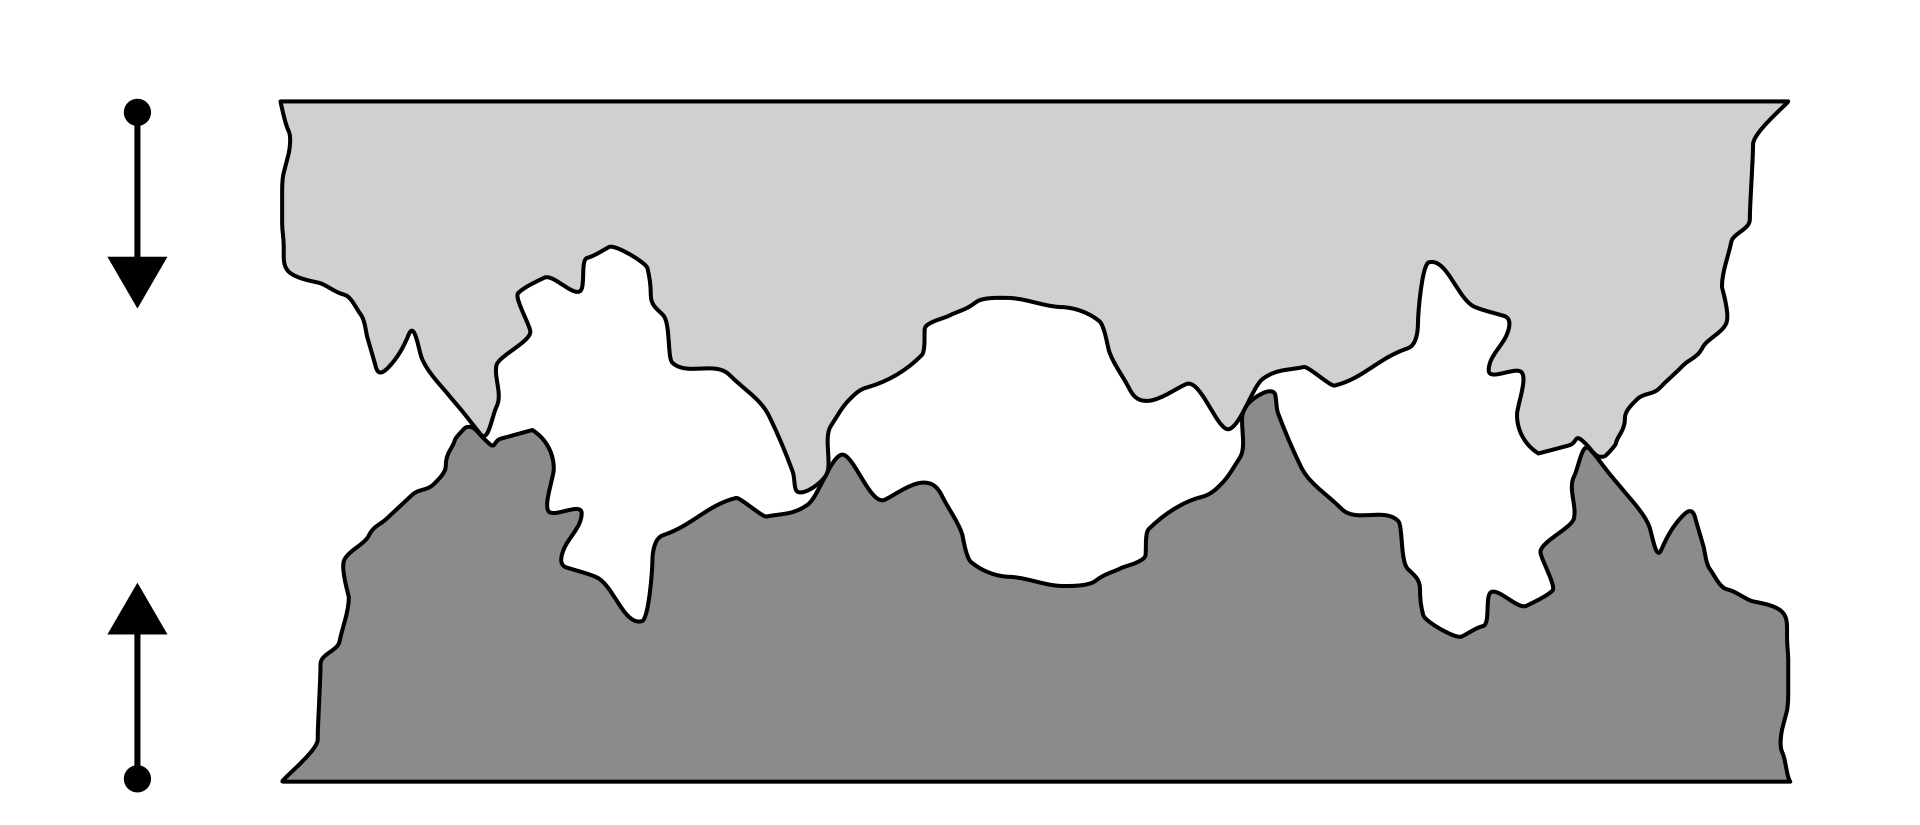
\includegraphics[width=\textwidth]{figures/theory/asperities_top.png}
      \caption{Low load.}
      \label{fig:asp_left}
  \end{subfigure}
  \hfill
  \begin{subfigure}[b]{0.49\textwidth}
      \centering
      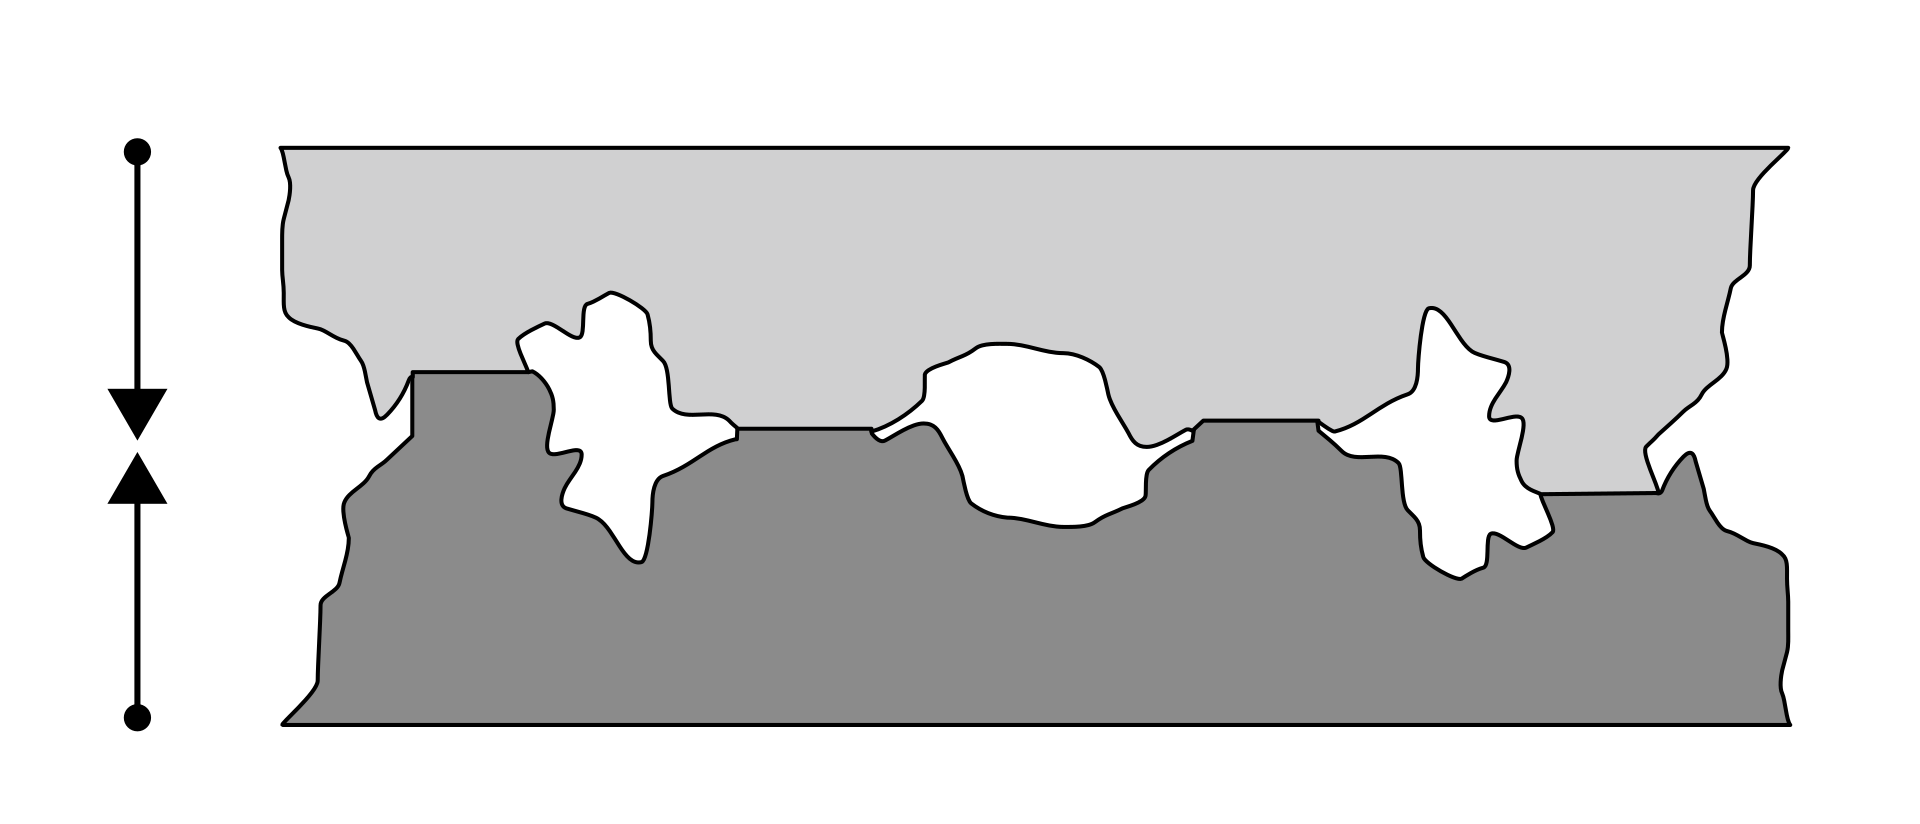
\includegraphics[width=\textwidth]{figures/theory/asperities_bottom.png}
      \caption{High load.}
      \label{fig:asp_right}
  \end{subfigure}
  \hfill
     \caption{Qualitatively illustration of the microscopic asperity deformation under increasing load from frame a to b \cite{wiki:asperities}.}
     \label{fig:asperity_contact}
\end{figure}
Many studies have focused on single asperity contacts to
reveal the relationship between the contact area and $F_N$ (13-15 from
\cite{mo_friction_2009}). By assuming perfectly smooth asperities, with radii of
curvature from micrometers all the way down to nanometers, continuum mechanics can be used to predict the deformation of asperities as normal force is applied. A model for non-adhesive contact between homogenous, isotropic, linear elastic spheres was
first developed by Hertz (17 from \cite{mo_friction_2009}), which predicted
$A_{\text{asp}} \propto F_N^{2/3}$. Later adhesion effects were included in a
number of subsequent models, including Maugis-Dugdale theory (18 from
\cite{mo_friction_2009}), which also predicts a sublinear relatinship between
$A_{\text{asp}}$ and $F_N$. Thus, the common feature of all single-asperity theories is that $A_{\text{asp}}$ is a sublinear function of $F_N$, leading to a similar sublinear relationship for $F_\text{fric}(F_N)$, which fails to align with the macroscale observations modelled by Amontons’ law (eq. \eqref{eq:amonton}).

A variety of multiasperity theories has attempted to combine single asperity mechanics by statistical modelling of the asperity height and spatial distributions \cite{CARBONE20082555}. This has led to ... a linear relationship between $A_{\text{asp}}$ and $F_N$. Unfortunately, these results are restricted in terms of the magnitude of the load and contact area, where multiasperity contact models based on the original ideas of Greenwood and Williamson \cite{GW} only predicts linearity at vanhising low loads, or Persson \cite{Persson} which works for more reasonable loads but only up to 10-15 \% of the macroscale contact area. However, as the load is furhter increased all multiasperity models predict the contact area to fall into the sublinear dependency of normal force as seen for single aperity theories \cite{CARBONE20082555}.




% Other authors proposed an empirical model in which mechanics of a nanoscale non-adhesive contact is controlled by load, that is, $F_f = \mu L$ and the contact area is undefined and unnecessary5,29 \cite{mo_friction_2009}

% \cite{mo_friction_2009} agues that the break-down of single-asperity theories of friction is due to the asperity (circumfereance defined) area is not proportional to the real one. By obtaining the real area (contacting bond) he arrives at the macroscale relationship... Quote: As shown in Table 1, friction force is now proportional to contact area at all length scales as long as the contact area is correctly defined at each length scale. When adhesion is added they arrive at the sublinear trend again. 


% \hl{What about multi asperity theory?}

% Our model predicts that as the adhesion between the contacting surfaces is reduced, a transition takes place from nonlinear to linear dependence of friction force on load. \cite{mo_friction_2009}




% This approach enables the bottom-up derivation of the linear scaling laws of macroscopic friction with size, and their transition to the sublinear ones for incommensurate nanosized contacts. We can now understand that such transition takes place when the contact roughness becomes large compared to the range of interfacial interactions [162] \cite{Manini_2016}.


% However, practical single- and multiplecontact conditions are characterized by
% complex interaction profiles plus nontrivial internal dynamics. As a result,
% the interplay of thermal drifts, contact ageing, contact-contact interactions,
% and macroscopic elastic deformations introduce significant complications, and
% make the depinning transition from static to kinetic friction an active field
% of research. \cite{Manini_2017}[p. 2]. 



% However, even though the successes of continuum mechanics there is no reasion to
% believe that it will be capable of reproducing tribological behaviour at the
% nanometre length scale where the discreteness of atoms often has a direct effect
% on physical properties \cite{Szlufarska_2008}.

\subsection{Nanoscale - Atomic scale}
Going from a micro- to nanoscale, on the order of $10^{-9}$ meter, it has been
predicted that continnum mechanics will break down \cite{luan_breakdown_2005}
due to the discreteness of individual atoms. Note that atom spacing lies in the
domain of a few ångströms Å ($10^{-10}$ m) and thus we take the so-called
corresponding atomic-scale to be a part of the nanoscale regime. In a numerical
study by Mo et al. \cite{mo_friction_2009} (considering asperity radii of 5-30
nm) it has been shown that the asperity area $A_{\text{asp}}$, defined by the
circumfereance of the apparent asperity contact zone, is in fact sublinear with
$F_N$. This is accommodated by the observation that not all atoms within the
circumfereance make chemical contact with the substrate. By
modelling the real area $A_{\text{real}} = NA_{\text{atom}}$, where $N$ is the
amount of atoms within the range of chemical interaction range and
$A_{\text{atom}}$ is the associated atom surface area, they found a consistent
linear relationship between friction and the real contact area. Without adhesive
forces this lead to a similar linear relationship $F_{\text{fric}} \propto F_N$,
while adding van der Waals adhesion to the simulation gave a sublinear
relatinship, even though the $F_{\text{fric}} \propto A_{\text{real}}$ was
maintained. 

This result emphasizes that contact area is still expected to be play a
major role on the nanoscale for asperity theory. It is simply the definition of contact area that undergoes a change when transistioning from micro- to
nanoscale. However, considering the simulation setup of our numerical study, a
flat sheet on a flat substrate, it is unfounded to rely on asperity theories. With no asperities present it is unknown (I could not find anay articles on contact area
for nanoflakes) whether the real contact area continue to be dominant part of the friction mechanism at play. Before diving into alternative theoretical approaches to adress this issue we point out that we might in fact be able to introduce an ensemble of asperities through a strategic combination of kirigami inspired cuts and stretching of the sheet. Hence, we might hypothesize that such a transsition will contribute to significant change in the goverening mechanism of friction in the system which we attempt to optimize for certain properties.
\\
\\
In the lack of noteworthy structural asperities on, the friction can instead be modelled as a consequencse of the rough potential of the atomic landscape. A series of models builds on this idea by considering different ways for the atoms to interact interatomic, with the moving body and the substrate surface. In figure \ref{fig:PT_FK_FKT} three major models 1D models is displayed. The time-honered  Prandtl-Tomlinson (PT) model describes a point-like tip sliding over a space-periodic fixed crystalline surface with a harmonic coupling to the \textit{moving body}. This is analog to that of an experimental cantilever (experimental name). Further extensions was added in the Frenkel-Kontorova (FK) model by substituting the tip with a chain of harmonic coupled atoms dragged from the end (I am not sure that the figure is correct here by drawing a spring), and finally combinned in the Frenkel-Kontorova-Tomlinson (FKT) with the addition of a harmonic coupling between the chain and the moving body.

\begin{figure}[H]
  \centering
  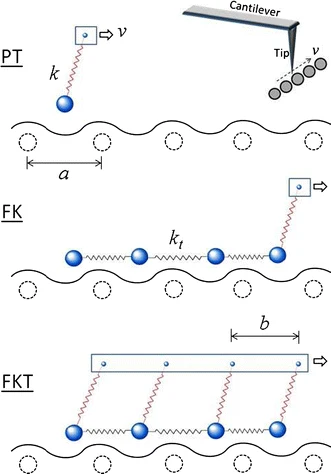
\includegraphics[width=0.4\linewidth]{figures/theory/PT_FK_FKT.png}
  \caption{\hl{Temporary} figure from \url{https://www.researchgate.net/figure/llustrations-of-the-1D-PT-FK-and-FKT-models-Large-solid-spheres-represent-tip-atoms_fig1_257670317}}
  \label{fig:PT_FK_FKT}
\end{figure}



% \hl{Search for experimental and numerical studies of nanoflakes (ideally with graphene) to talk about expectations here.} 








% Our results confirm the conclusions of other authors that single-asperity theories break down at the nanoscale1,5. \cite{mo_friction_2009}


% Experimental research to examine the frictional characteristics at the
% atomic-scale has been conducted for the past two decades. It is well known
% that frictional behavior cannot be generalized by a few factors such as normal
% load, surface roughness, speed, and material type of the tribological system.
% Other conditions such as temperature, humidity, and even sliding history can
% affect the tribological phenomena significantly. Particularly at nano-scale,
% the tribological behavior tends to be more sensitive to the state of outermost
% layer of the surface region. Thus, contamination layer, adsorbed gas,
% capillary junctions, and oxide layer become more important at small scales.
% This is because at nano-scale the contact forces are often too low for the
% asperities to penetrate the surface layers and the magnitude of the surface
% force may be comparable to the frictional force. {kim_nano-scale_2009}.


% Together with the current experimental possibility to perform well-defined
% measurements on well-characterized materials at the fundamental microscopic
% level of investigation of the sliding contacts, advances in the computer
% modeling of interatomic interactions in materials science and complex systems
% encompass molecular-dynamics (MD) simulations of medium to large scale for the
% exploration of the tribo-dynamics with atomic resolution [4, 5].




% \subsubsection{Tomlinson model}
% % \cite{kim_nano-scale_2009}

% One of the first atomic scale models. Here we have no asperities but it is based on the assumptions that the atomic surface is not completely smooth. Since atoms was modelled as spheres the surface topography would not be completely flat. The idea is shown in figure \ref{fig:tomlinson_model} where the moving body is connected the atom with springs.
% \begin{figure}[H]
%   \centering
%   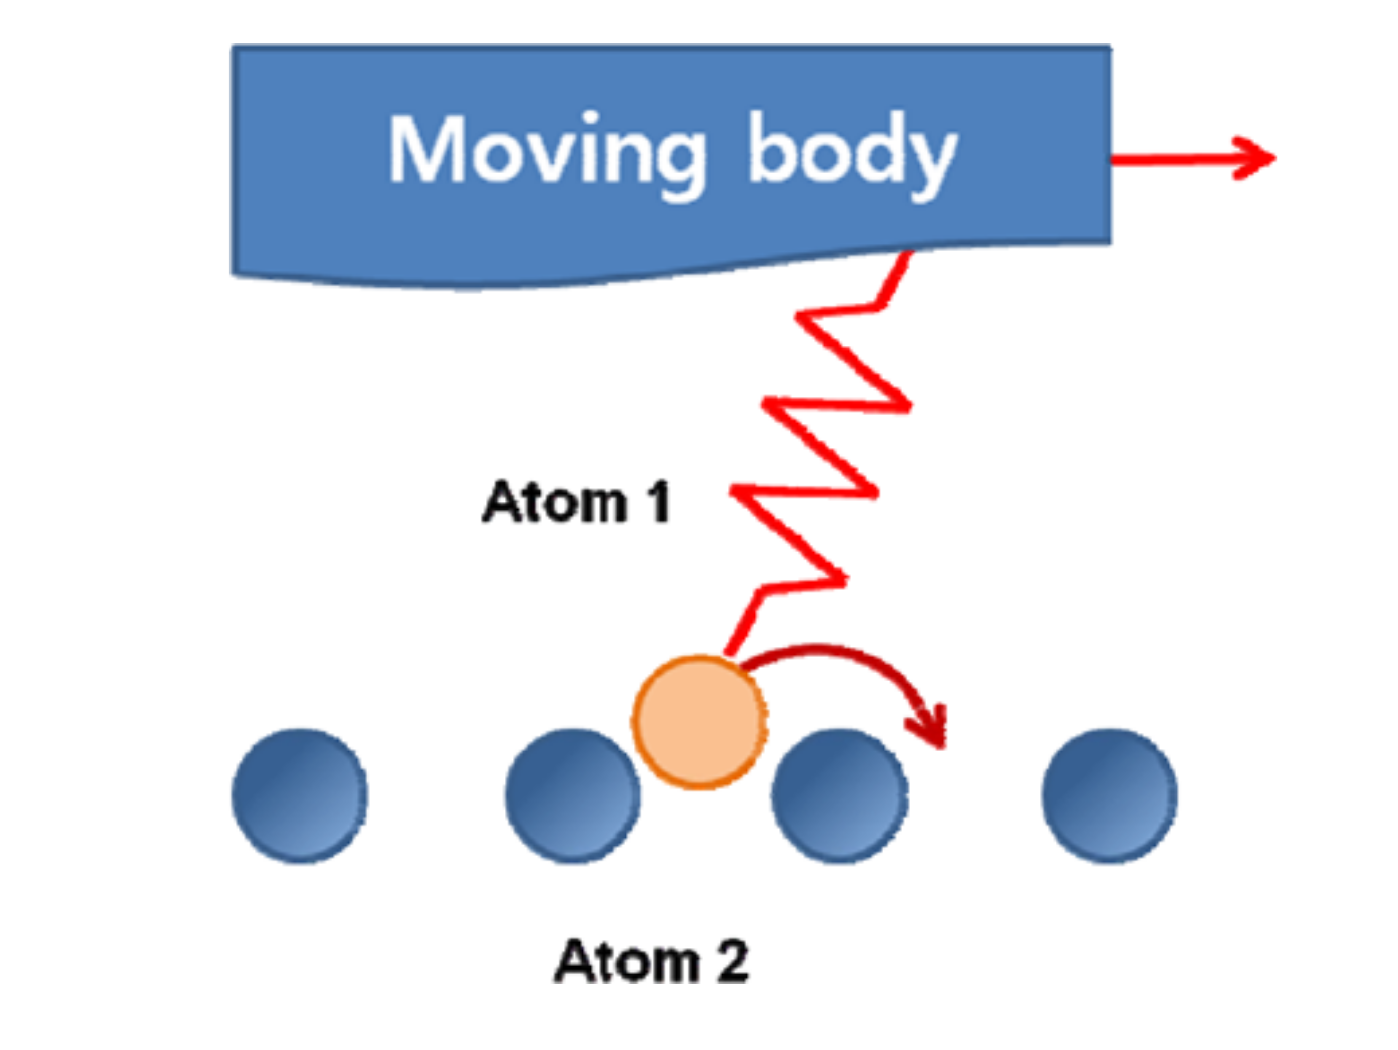
\includegraphics[width=0.5\linewidth]{figures/theory/tomlinson_model.png}
%   \caption{\hl{Temporary} figure from \cite{kim_nano-scale_2009}}
%   \label{fig:tomlinson_model}
% \end{figure}


% This model gives an explanation to the stick-slip behaviour. This layed the foundation for the Frenkel-Kontorova model so maybe go straight to that?

\subsubsection{Frenkel-Kontorova}
% Based on \cite{Manini_2016} and \cite{FK2D}.

The standard Frenkel-Kontorova (FK) model consists of a 1D chain of $N$ classical
particles of equal mass, representing atoms, interacting via hamornic forces and moving in a sinusoidal potential as sketched in figure \ref{fig:FK_model}. The hamiltonian
is 
\begin{align}
  H = \sum_{i=1}^N \left[\frac{p_i^2}{2m} + \frac{1}{2}K(x_{i+1} - x_i - a_c)^2 + \frac{1}{2}U_0 \cos{\left(\frac{2\pi x_i}{a_b}\right)}\right],
  \label{eq:H_FK}
\end{align}
where the atoms are labelled sequently $i = 1, \hdots, N$. The first term $p_i^2/2m$ represents the kinetic energy with momentum $p_i$
and mass $m$. Often the effetcs of inertia are neglected, reffered to as the static FK model, while the inclusion, as shown in eq.~\eqref{eq:H_FK}, is known as the dynamic FK model \cite{FK2D}. The next term describes the harmonic interaction with elastic
constant $K$, nearest neighbour distance $\Delta x = x_{i+1} - x_i$ and 
corresponding nearest neighbour equilibrium distance $a_c$. The final term represents the periodic substrate potential (external potential on site) with amplitude $U_0$ and period $a_b$. Different boundary choices can be made where both free ends nad periodic conditions gives reasonable results. The choice of fixed ends however makes the chain incapable of sliding.


\begin{figure}[H]
  \centering
  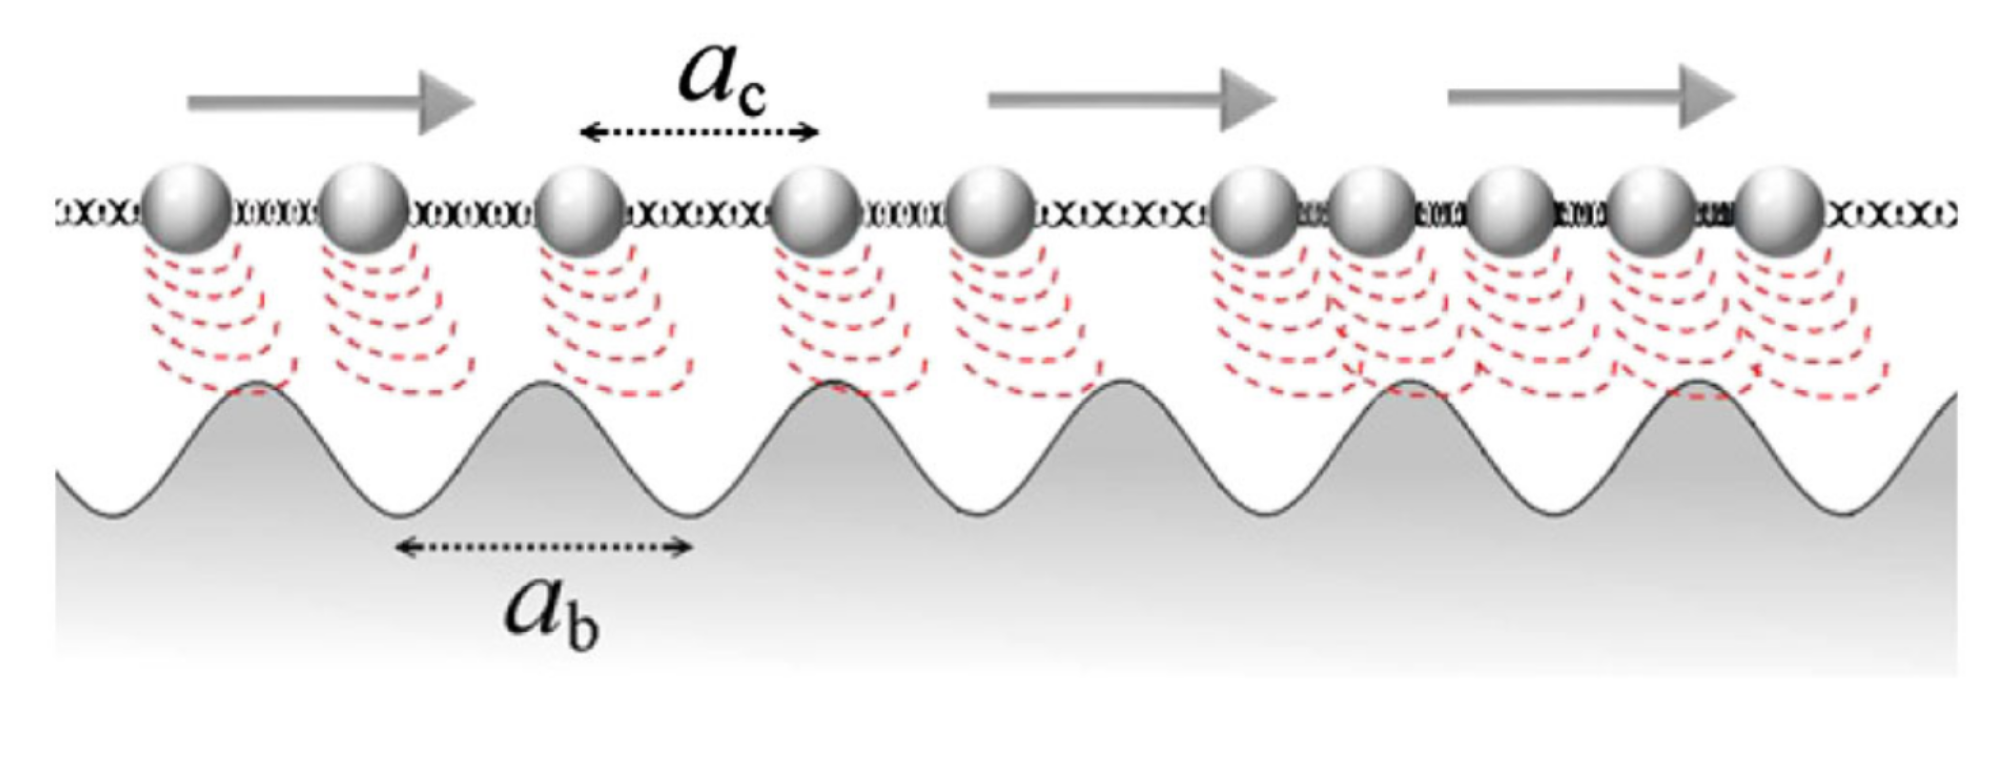
\includegraphics[width=0.8\linewidth]{figures/theory/FK_model.png}
  \caption{\hl{Temporary} figure from \cite{Manini_2016}}
  \label{fig:FK_model}
\end{figure}

To probe static friction one can apply an external force which increases adiabatically until sliding accours. This corresponds to the static FK model and it turns out that the sliding properties are entirely governed by its topological excitations referred to as so-called \textit{kinks} and \textit{antikinks}

\paragraph*{Commensurability} We can describe the frictional behvaiour in terms of commensurability, that is, how well the spacing of the atoms match the periodic substrate potential. We describe this by the length ratio $\theta = a_b / a_c = N / M$ where $M$ denotes the number of minemas in the potential (within the length of the chain). A rational number for $\theta$ means that we can align the atoms in the chain perfectly with the minemas, without stretching the chain, corresponding to a \textit{commensurate} case. If $\theta$ is irrational the chain and substrate cannot fully align, and we denote this as being \textit{incommensurate}.

We begin with the simplest commensurate case of $\theta = 1$ where the
spacing of the atoms matches perfectly the substrate potential periodicity, i.e.
$a_c = a_b$, $N = M$. The ground state (GS) is the configuration where each atom
fits in one of the substrate minema. By adding an extra atom we would effectively
shift over some atoms, away from these ideal state, giving rise to a kink excitation, i.e. two atoms will have to share the same potential corrugation as
sketched in figure \ref{fig:incommensurable_example}.  On the other hand, removing an atom from the chain results in a antikink excitation where one potential corrugation will be left ``atomless''. In order to reach a local minimum the kink
(antikink) will expand in space over a finite length such that the chain undertakes a local compression (expansion). When applying a tangential force to the
chain it is much easier for a kink to move along the chain than it is for the non-exicted atoms since the activation energy $\epsilon_{PN}$ for a kink displacement is systematically smaller (often much smaller) than the potential barrier $U_0$. Thus, the motion of kinks (antikinks), i.e. the displacement of extra atoms (atom vacancies), is represententing the fundamental mechanism for mass transport. These displacements is responsible for the mobility, diffusivity and conductivity within this model. 

In the ideal zero temperature commensurable case with an adiabatical increase in force, all atoms would be put into an accelerating motion as soon the lowest energy $NU_0$ is present. However, in reality any thermal excitation would excite the system before this point is reached by the creation of kink-antikink pairs that would travel down the chain. For a chain of finite length these often accour at the end of the chain running in opposite direction. As a kink travels down the chain the atoms is advanced by one atom spacing $a_b$ along the substrate potential. This cascade of kink-antikink exications is shown in figure \ref{fig:kink_antikink}

\begin{figure}[H]
  \centering
  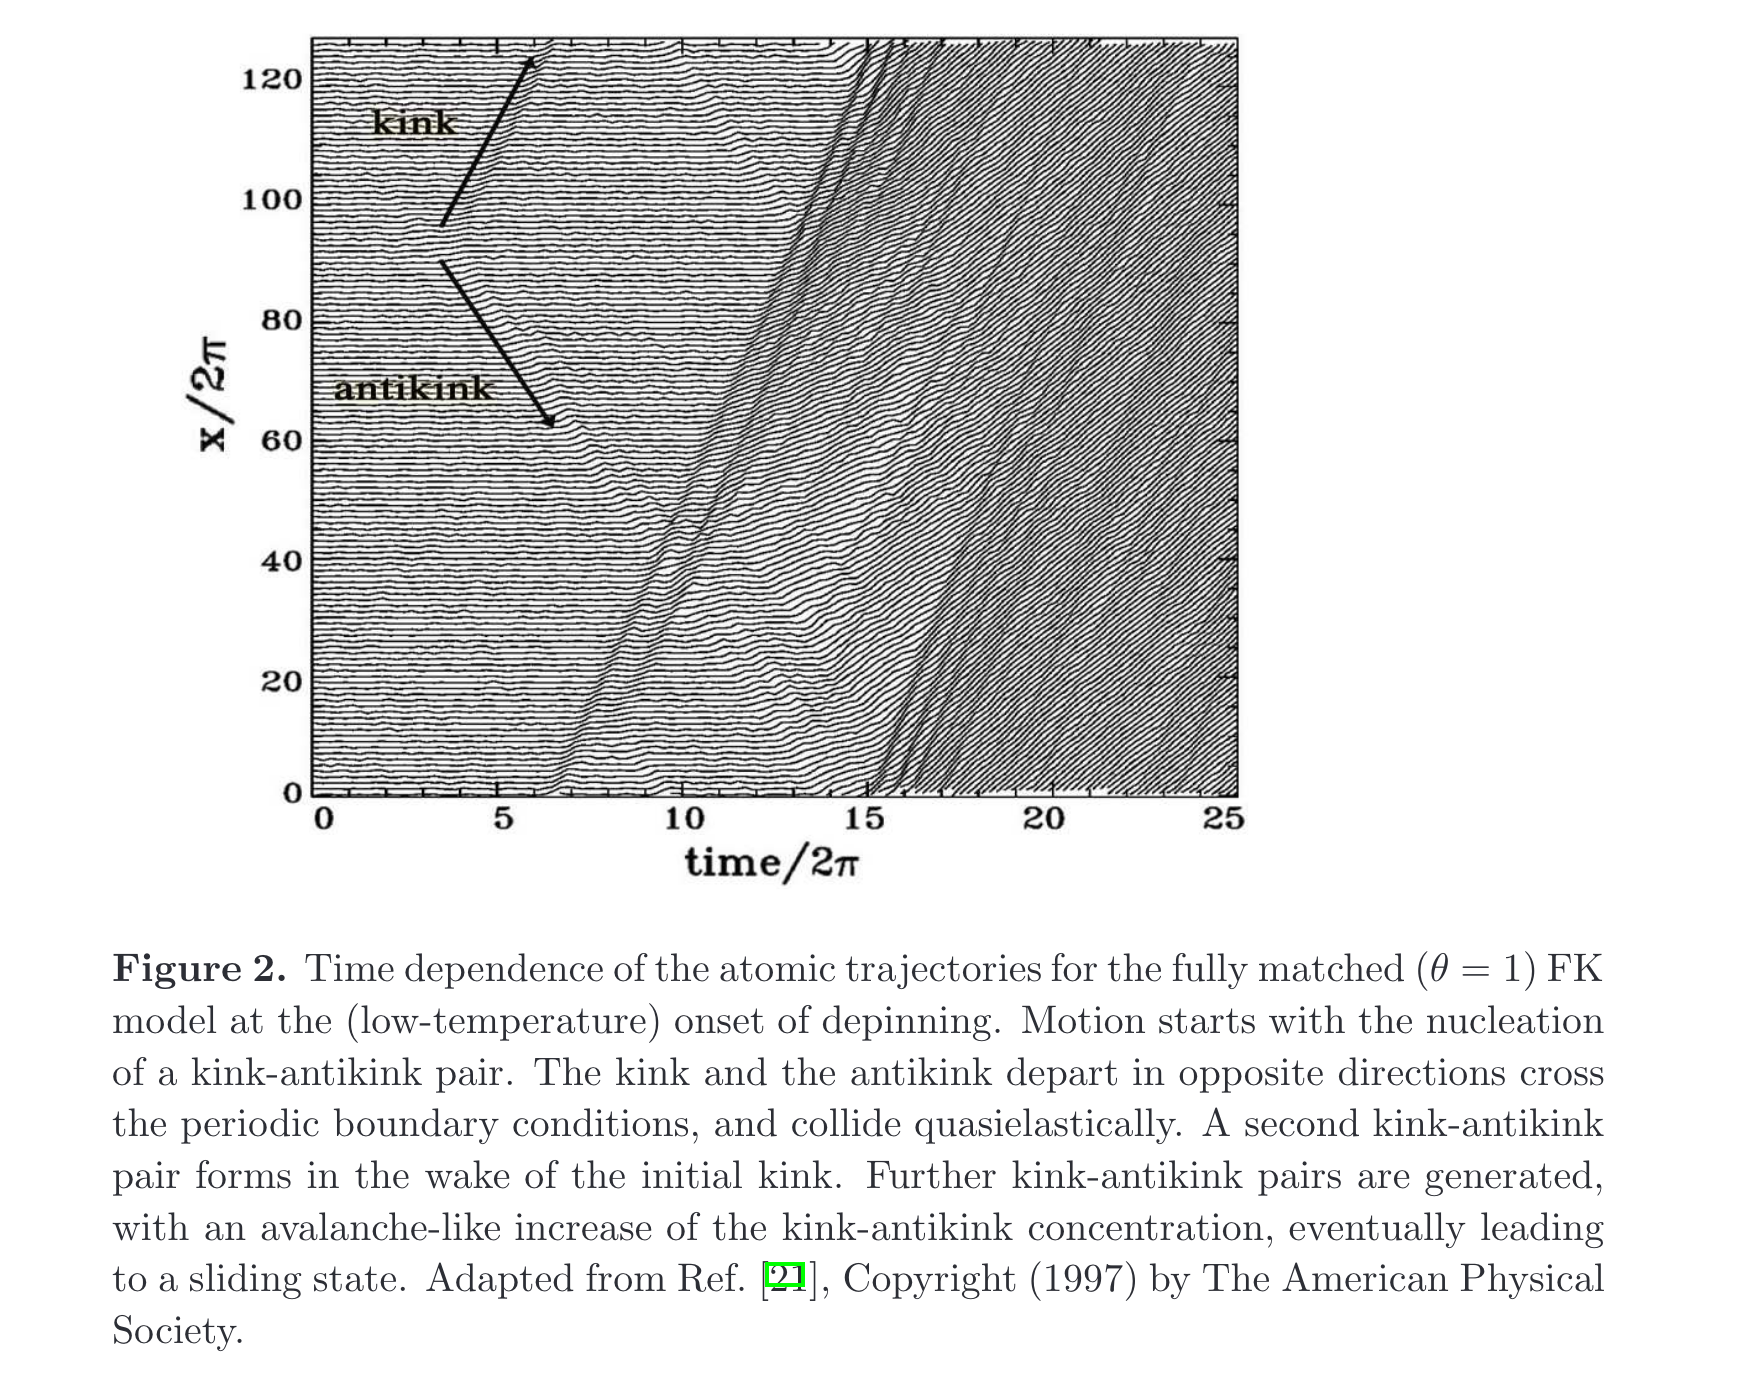
\includegraphics[width=0.8\linewidth]{figures/theory/kink_antikink.png}
  \caption{\hl{Temporary} figure from \cite{Manini_2016}}
  \label{fig:kink_antikink}
\end{figure}

For the 2D case where an island is deposited on a surface, in our case the graphene sheet on the Si substrate, we generally also expect the sliding to be initated by kink-antikink pairs at the boundary. 

For the case of incommensurability, i.e. $\theta = a_b/a_c$ is irrational, the
GS is characterized by a sort of ´´staircase'' deformation. That is, the chain
will exhibit regular periods of regions where the chain is slightly compressed
(expanded) to match the substrate potential, seperated by kinks (antikinks),
where the increased stress is eventually released through a localized expansion
(compression) as illustrated in figure \ref{fig:incommensurable_example} \hl{Go though this again and make sure that I got the compression expansion directions rihgt...}.

\begin{figure}[H]
  \centering
  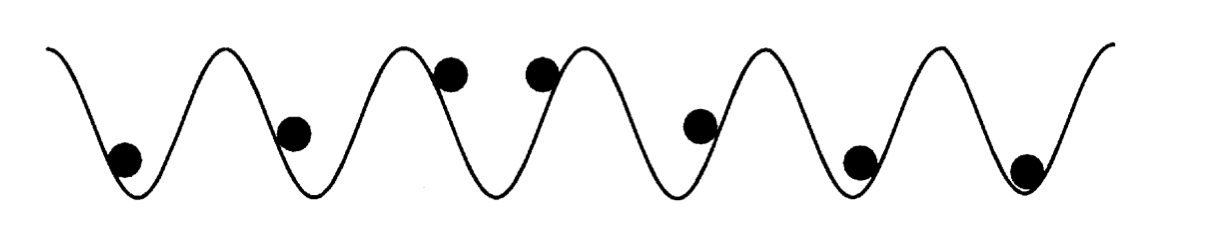
\includegraphics[width=0.5\linewidth]{figures/theory/incommensurable_example.png}
  \caption{\hl{Temporary} figure from
  url{http://www.iop.kiev.ua/~obraun/myreprints/surveyfk.pdf} p. 14.
  Incommensurable case ($\theta = ?$) where atoms sits slightly closer than
  otherwise dictated by the substrate potential for which this regularly result
  in a kink here seen as the presence of two atoms closeæy together in on of the
  potential wells.}
  \label{fig:incommensurable_example}
\end{figure}

% Maybe use the strength $\lambda = U_0 / (K a_b^2)$ with critical strength $\lambda_c$ instead of critical $K$?

The incommensurable FK model contains a critical elastic constant $K_c$, such
that for $K > K_c$ the static friction $F_s$ drops to zero, making the chain able to initiate a slide at no energy cost, while the low-velocity kinetic friction is dramatically reduced. This can be explained by the
fact that the displacement accouring in the incommensurable case will yield just
as many atoms climbing up a corrugation as there are atoms climbing down. For an
infinite chain this will exactly balance the forces making it
non-resistant to sliding. Generally, incommensurability guarantees that the
total energy (for $T=0$) is independent of the relative position to the
potential. However, when sliding freely a single atom will eventually occupy a
maximum of the potential. When increasing the potential magnitude $U_0$ or
softning the chain stiffness, lowering $K$, the possibility to occupy such a
maximum is no longer present. This marks the so-called \text{Aubry transition}
at the critical elasric constant $K = K_c(U_0, \theta)$ where the chain goes
from a free sliding to a \textit{pinned state} with a nonzero static friction.
$K_c$ is a discontinuous function of the ratio $\theta$, due to the reliance on
irrational numbers for incommensurability. The minimal
value $K_c \simeq 1.0291926 $ in units $[2 U_0 (\pi / a_b)^2]$ is achieved for
the golden-mean ratio $\theta = (1+\sqrt{5}/2)$. Notice that the pinning is
provided despite translational invariance due to the inaccessibility to move
past the energy barrier which act as dynamical constraint. The Aubry transistion
can be invistigated as a first-order phase transistion for which power laws can be
defined for the order parameter. This is beyond the scope of this thesis as we
merely are going to point to the FK model for the understanding of stick-slip
behvaiour and the concept of commensurability.

The phenonema of non-pinned configurations is named \textit{superlubricity} in
tribological context. Despite the misleadning name this referes to the case
where the static friction is zero while the kinetic friction is nonzero but
reduced. For the case of a 2D sheet it is possible to alter the commensurability
by changing the orientation of the sheet relative to the substrate. This has
been shown for a graphene flake (single layer) sliding over a graphite surface
(multiple layers) \cite{DIENWIEBEL2005197}. In figure \ref{fig:graphene_rot} we see how the friction depends on the relative orientatin between the sheet and substrate.


\begin{figure}[H]
  \centering
  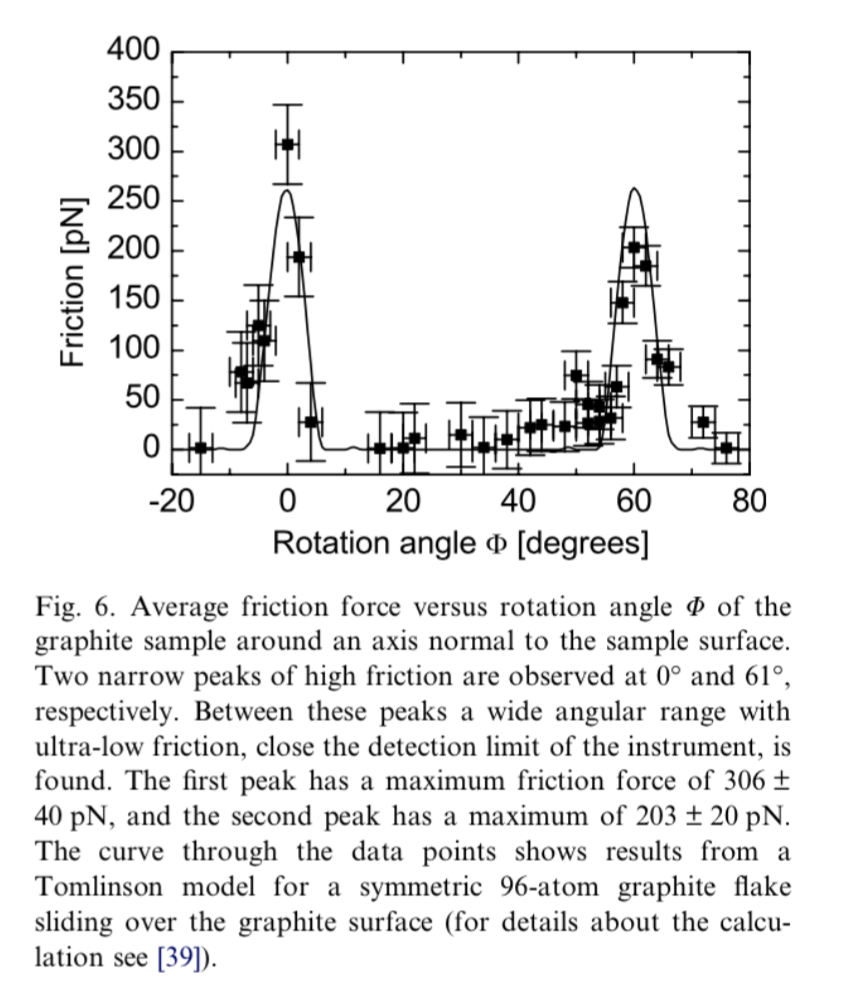
\includegraphics[width=0.5\linewidth]{figures/theory/graphene_rot.png}
  \caption{\hl{Temporary} figure from \cite{DIENWIEBEL2005197} showing superlubricity for incommensurable orientations between graphene and graphite. \hl{temporary}}
  \label{fig:graphene_rot}
\end{figure}



\paragraph*{Kinetic friction}
% Maybe check out for more info on the 1D model: Y. S. Kivshar O. M. Braun. The Frenkel-Kontorova Model. Springer, 1st edition, 2004.

%Based on \cite{FK2D}


% The FK model can also describe phonons and heat in the lattices, which absorb the kinetic energy of the sliding[4]. \cite{FK2D}

% Consequently, the FK model is the simplest model in which dynamic friction is emergent, while in other models some form of heuristic damping must be included.\cite{FK2D}

In the FK model the kinetic friction is primarily caused by resonance between
the sliding induced vibrations and phonon modes in the chain \cite{FK2D}. When all atoms are sliding rigidly width center of mass velocity $v_{{\text{CM}}}$ the atoms will pass the potential maxima with the so-called \textit{washboard frequency} $\Omega = 2\pi v_{{\text{CM}}} / a_b$. For a weak coupling between the chain and the potential we can use the zero potential case as an approximation for which the known dispersion relation for the 1D harmonic chain is given [Kittel]
\begin{align*}
  \omega_k = \sqrt{\frac{4 K}{m}} \left|\sin{\left(\frac{k}{2}\right)}\right|,
\end{align*}
where $omega_k$ is the phonon frequency and $k = 2\pi i / N$ the wavenumber with $i\in [N/2, N/2)$. Strong resonance will accour if $\Omega$ is close to the frequency of the phonon modes $\omega_q$ in the chain with wavenumber $q = 2\pi a_c / a_b = 2\pi \theta^{-1}$ or its harmonics $nq$ for $n = 1, 2, 3, \hdots$ \cite{van_den_Ende_2012}. Thus, we can approximate the resoancne speed as s
\begin{align*}
    n \Omega &\sim \omega_{nq} \\
    n \frac{2\pi v_{\text{CM}}}{a_b} &\sim 2 \sqrt{\frac{K}{m}} \left| \sin{\left(\frac{2n \pi \theta^{-1}}{2}\right)}\right| \\
    v_{\text{CM}} &\sim \frac{\sin{(n\pi \theta^{-1})}}{n \pi} \sqrt{\frac{Ka_b^2}{m}}.
\end{align*}
When the chain slides with a velocity around resonance speed, the washboard frequency can excite acoustic phonons which will dissipate to other phonon modes as well. At zero temperature the energy will transform back and forth between internal degrees of freedom and center of mass movement of the chain. Hence, at zero temperature this will infact speed up the translation decay (decay is synonymous for translational movement right?). However, for the more realistic case of non-zero temperature the substrate serves as a thermostat for which energy will dissipate from the chain to the substrate degrees of freedom giving rise to kintetic friction. On the other hand, this predicts that certain sliding speed, which does not induce phonon resossance, will be subject to extremely low kinetic friction. This is strongly connected to the superlubricity term although ths phonon dynamics is simplified in this 1D model. 

A common way to model the non-zero temperature case is by the
use of a Langevin thermostat, which simulates the dissipation by adding a viscous
damping force and thermal fluctuations by the addition of Gaussian random forces
with variance proportional to the temperature (This is covered in more details
in section \ref{sec:langevin}). In combinatio, this gives rise to a kinetic friction that is both velocity and temperature dependent. 

By extending the FK model into 2D \cite{FK2D} it can be shown numerically that the friction coefficient generally increases with increasing velocity and temperature resepectively. 


% Simulations of concentric nanotubes in relative motion (telescopic sliding), have revealed the occurrence of well-defined velocities at which friction is enhanced, corresponding to a washboard frequency resonating with longitudinal [172] or circular [173] phonon modes, leading to enhanced energy dissipation. The frictional response becomes highly non-linear while approaching the critical velocity and, contrary to macroscopic systems, washboard resonances can arise at multiple velocities, especially for incommensurate interfaces where more than one length scale may be in common to the contacting surfaces [172] \cite{Manini_2016}.




% As the system is Hamiltonian (no heuristic damping) the total energy is conserved. Nevertheless, energy can be transferred from the centre of mass to the internal degrees of freedom, leading to the arrest of the chain in time. This effect can be interpreted as an effective friction. \cite{van_den_Ende_2012}


% The majority [6–12] examines the steady state of the dynamical FK model in the presence of dissipation, rep- resenting the coupling of phonons to other, undescribed degrees of freedom. \cite{PhysRevLett.85.302}


% Static friciton behvaiour is robust and remains similar in 2D but dynamical friction is strongly influenced. 




% When considering the nonzero temperature thermal fluctuations can then overcome pinning effects even in fully commensurate cases.



% By applying a finite driving force it is known that a pinned configuration will go through several first-order dynamical pahse transistions as the system transfers from a pinned to a sliding state. 



% At face value, the transition from a static strained configuration to full
% sliding is conceptually as simple as overcoming an energy barrier. However,
% practical single- and multiple- contact conditions are characterized by
% complex interaction profiles plus nontrivial internal dynamics. As a result,
% the interplay of thermal drifts, contact ageing, contact-contact in-
% teractions, and macroscopic elastic deformations introduce significant
% complications, and make the depinning transition from static to kinetic
% friction an active field of research. The depinning dynamics affects in
% particular the transition between stick-slip and smooth slid- ing for sliding
% friction. (Current trends in the physics of nanoscale friction)


% In Atomic Force Microscopy (AFM) experiments, when the tip scans over the
% monolayers at low speeds, friction force is reported to increase with the
% logarithm of the velocity, similar to that observed when the tip scans across
% crystalline surfaces. This velocity dependence is interpreted in terms of
% thermally activated depinning of interlocking barriers involving interfacial
% atoms. (Current trends in the physics of nanoscale friction)




% \begin{enumerate}
%   \item Properties depending on $\Theta = N/M = a_b/a_c$
%   \item Elastic constant $K$
%   \item Kinks anti kinks travelling
%   \item Importance of commensurability between lattice and potential 
%   \item Aubry transition
%   \item Pinning and unpinning, stick slip
%   \item superlubricity (no stick slip, but still kinetic friction)
%   \item Adding a Langevin thermostat on top of this introduces temperature. 
%   \item Phase transistion?
% \end{enumerate}







% \subsubsection{FK extension: Frenkel-Kontorova-Tomlinson (FKT)}

% Further model extensions. Important? 
% Several extensions has been provided for the FK model with modifications of the
% interactions or system dimensionality. Anharmonicity of the chain 


% However, Weiss and Elmer (1995) proposed that the model had a deficiency. They suggested that in the FK model, there was no connection between the atoms and the sliding body. Therefore, Frenkel-Kontorova-Tomlinson (FKT) model that combines the FK model with the Tomlinson model was proposed. \cite{kim_nano-scale_2009}


% The Frenkel-Kontorova-Tomlinson (FKT) model [61, 62] introduces an harmonic
% coupling of the sliding atomic chain to a driving support, thus making it
% possible to investigate stick-slip features in a 1D extended simplified
% contact. The FKT framework provided the ideal platform to investigate the
% tribological consequences of combined interface incommensurability,
% finite-size effects, mechanical stiffness of the contacting materials, and
% normal-load variations \cite{Manini_2016}.


% Important generalizations involving increased dimensionality compared to the
% regular FK model bear significant implications for tribological properties
% such as critical exponents, size-scaling of the friction force, depinning
% mechanisms, and others. \cite{Manini_2016}

% Maybe check this out: An interesting example of such a transient is the
% depinning of an atomic monolayer driven across a 2D periodic substrate profile
% of hexagonal symmetry [83].  \cite{Manini_2016}


% \subsubsection{Other stuff}


% At nanoscales things get a bit more unclear. SFM (explain) experiments have
% reported (copy sources 5, 6, 21 from \cite{mo_friction_2009}) where $F_f \propto
% F_N$ or even with these quantities being nearly independent of each other.

% \cite{physicsworld_2005}

% Physically relevant quantities, including the average friction force, the slider and the lubricant mean velocities, several correlation functions, and the heat flow can be evaluated numerically by carrying out suitable averages over the model dynamics of a sliding interface, as long as it is followed for a sufficiently long time. The modeling of friction must first of all address correctly ordinary equilibrium and near-equilibrium phenomena, where the fluctuation-dissipation theorem (Sec. 2) governs the smooth conversion of mechanical energy into heat, but most importantly it must also deal with inherently nonlinear dissipative phenomena such as instabilities, stick-slip, and all kinds of hysteretic response to external driving forces, characteristic of non-equilibrium dynamics. 
% \cite{Manini_2016}


% In several works by J. Fineberg’s group [2–4] the transition from sticking to
% sliding is characterized by slip fronts propagating along the interface.
% \cite{Manini_2017}[p. 2]. 



% As expected, high levels of
% friction were present in the commensurate positions and extremely low friction
% was found when the surfaces were incommensurate.
% (\url{https://physicsworld.com/a/friction-at-the-nano-scale/})


% Superlubricity, now a pervasive concept of
% modern tribology, dates back to the math- ematical framework of the Frenkel
% Kontorova model for incommensurate interfaces [40]. When two contacting
% crystalline workpieces are out of registry, by lattice mismatch or angular
% misalignment, the minimal force required to achieve sliding, i.e. the static
% friction, tends to zero in the thermodynamic limit – that is, it can at most
% grow as a power less than one of the area – provided the two substrates are
% stiff enough. (Current trends in the physics of nanoscale friction)


% Superlubricity is experimentally rare. Until recently, it has been
% demonstrated or im- plied in a relatively small number of cases [29, 42–46].
% There are now more evidences of superlubric behavior in cluster
% nanomanipulation [32, 33, 47], sliding colloidal layers [48–50], and
% inertially driven rare-gas adsorbates [51, 52]. (Current trends in the physics
% of nanoscale friction)


% A breakdown of structural lubricity may occur at the heterogeneous interface
% of graphene and h-BN. Because of lattice mismatch (1.8\%), this interface is
% intrinsically incommen- surate, and superlubricity should persist regardless
% of the flake-substrate orientation, and become more and more evident as the
% flake size increases [57]. However, vertical cor- rugations and planar strains
% may occur at the interface even in the presence of weak van der Waals
% interactions and, since the lattice mismatch is small, the system can de-
% velop locally commensurate and incommensurate domains as a function of the
% misfit angle [58, 59]. Nonetheless, spontaneous rotation of large graphene
% flakes on h-BN is observed after thermal annealing at elevated temperatures,
% indicative of very low friction due to incommensurate sliding [60, 61].
% (Current trends in the physics of nanoscale friction)

% Indeed, we know from theory and simulation [74–76] that even in clean wearless
% friction experiments with perfect atomic structures, superlubricity at large
% scales may, for example, surrender due to the soft elastic strain deformations
% of contacting systems. (Current trends in the physics of nanoscale friction)



% \subsection{Multi scale models?}
% \cite{Manini_2016} p. 24.

\paragraph*{Temperature depence}

Might find something interesting here \cite{zhao_thermally_2007} or \cite{PhysRevE.71.065101}.


\paragraph*{Smooth sliding}

Find a suitable place to introduce smooth sliding. Above certain velocities the stick-slip motion dissapear. \cite[p. 142-ish]{gnecco_meyer_2015}

\subsubsection{Experimental procedures}
\cite{gnecco_meyer_2015}


Experimentally nanoscale friction is challenging to approach as the forces, on the scale of nano-newtons as well, is extremely small. Additionally surface topography is not easily viewed. On the other side simulations provide full transparency regarding information of the physical structure of the sample among with forces, velocities and temperature. However, in order to compare numerical results the experimental procedures is most often mirrored in simulations. Thus it is beneficial to adress the most common experimental techniques when designing a simulation. 

%  Not may nanoflake studies. 

\paragraph*{Scanning Probe Microscopy}

Scanning probe microscopy (SPM) includes a variety of experimental methods which
is used to examine surfaces with atomic resolution \cite[p.
6-]{BHUSHAN20051507}. This was orginally developed for surface topography
imaging, but today it plays a crucial role in nanoscale science as it is used
for probe-sampling regarding tribological, electronic, magnetic, biological and
chemical character. The famility of methods involving the measurement of forces
is generally referred to as \textit{scanning force microscopies} (SFM).

One such method arose from the \textit{atomic force micrpscope}, which consist
of a sharp micro-fabricated tip attacthed to a contilever force sensor, usually
with a sensitivy below 1 nN. The force is measured by recording the bending of
the cantilever, either as a change in electrical conduction or more commonly, by
a light beam reflected from the back of the cantilever into a photodetector
\cite{gnecco_meyer_2015}. By adjusting the tip-sample height to keep a constant
normal force while scanning accross the surface this can be used to produce a
surface topography map. By tapping the material (dynamic force microscopy) with sinusoidally vibrated tip the effects from friction and other disturbing forces can be minimized in order to produce a clear image (include example, preferable of graphene). However, when scanning perpendicularly to the cantilever
axis one is also able to measure the frictional force as torsion of the
cantilever. By having four quadrants in the photodetector (as shown in figure
\ref{fig:AFM}), one can simultaneously measure the normal force and friction
force as the probes scans accross the surface. 

\begin{figure}[H]
  \centering
  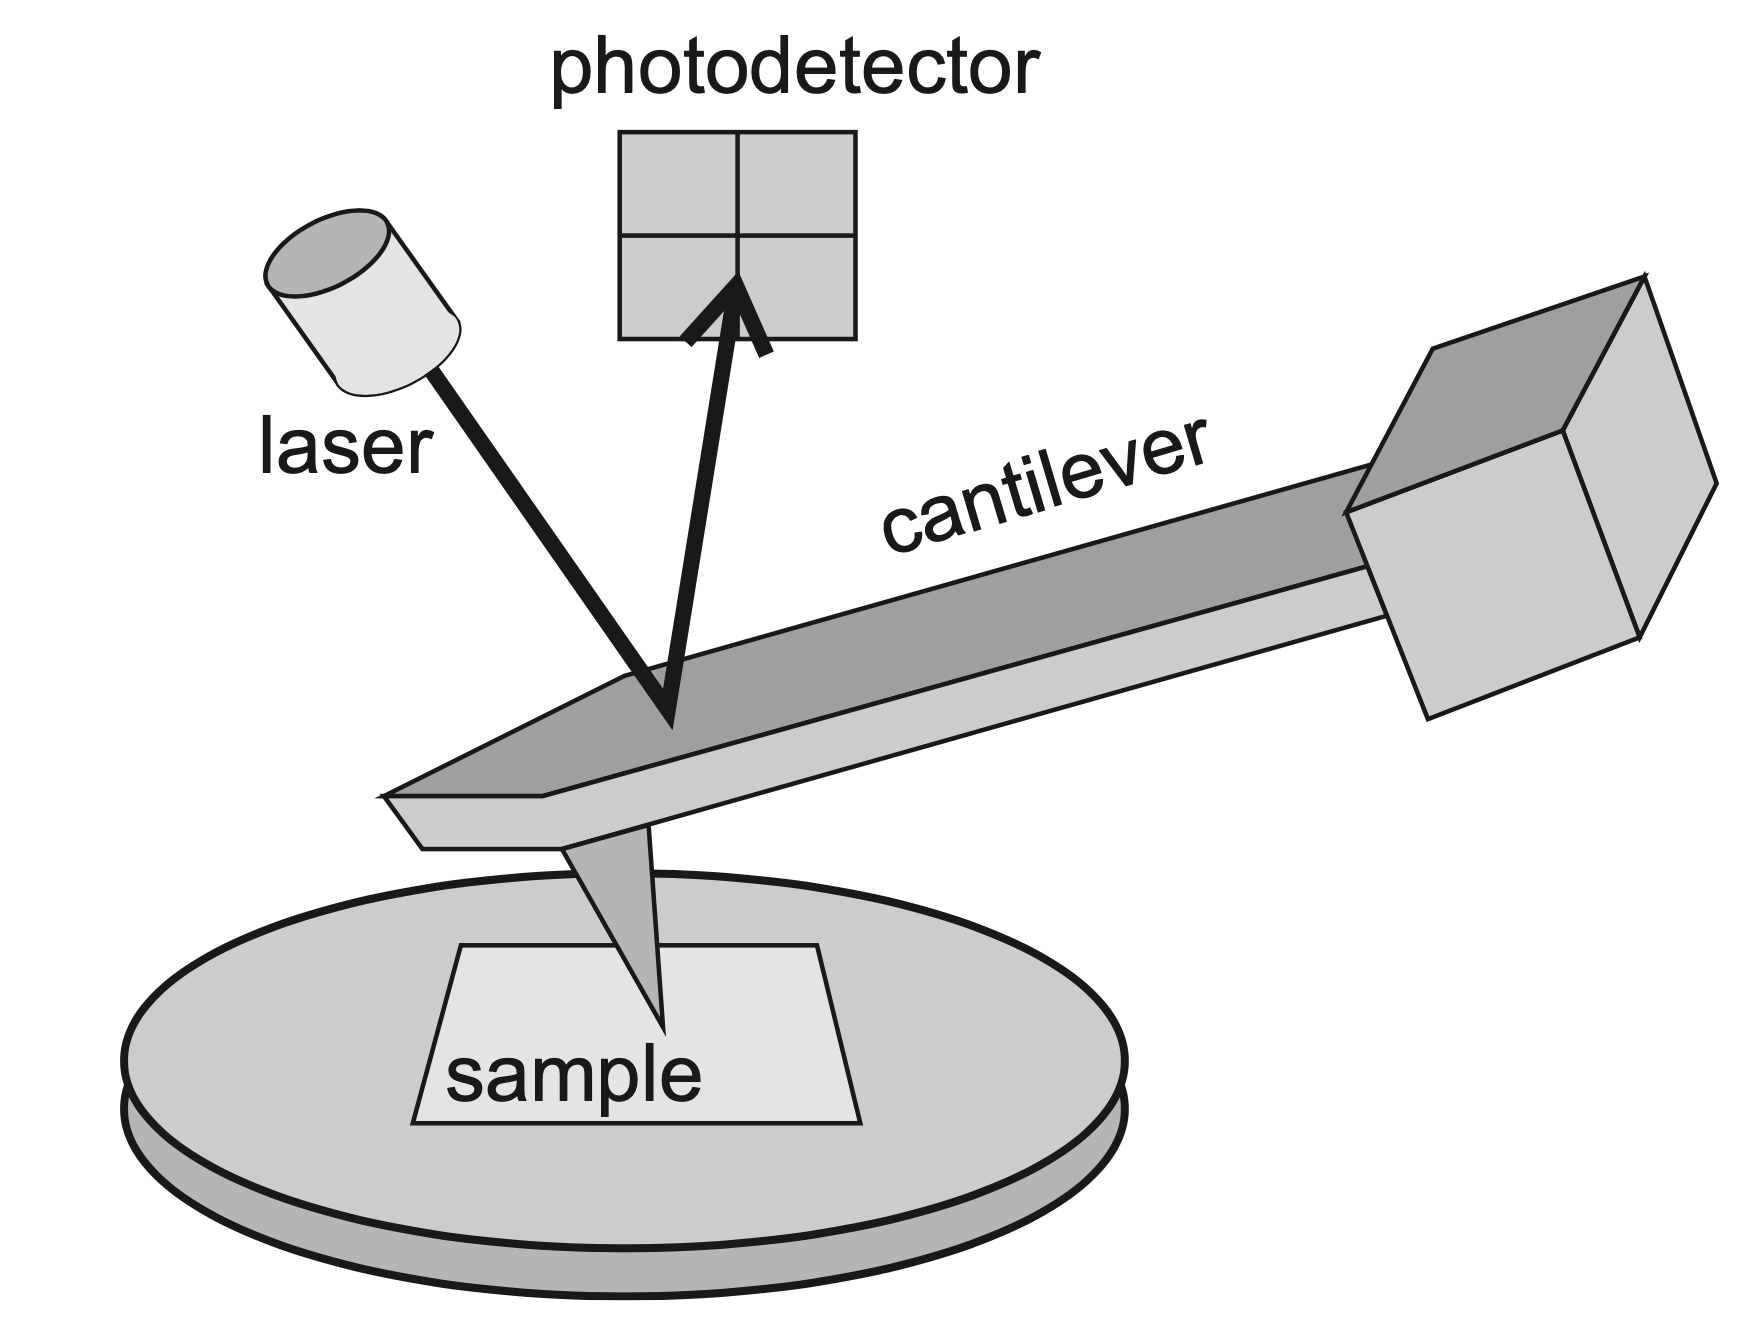
\includegraphics[width=0.6\linewidth]{figures/theory/AFM.png}
  \caption{\hl{Temporary} figure from \cite[p. 184]{gnecco_meyer_2015}}
  \label{fig:AFM}
\end{figure}


This can also be used to drag a nanoflake as done by Dienwiebel et al. \cite{DIENWIEBEL2005197} (earlier referrenced), where a graphene flake was attahced to a FFM tip and dragged accross graphite.




\paragraph*{Surface Force Apparatus (SFA)}

Is this the one where to surfaces slides in opposite direction (at least that is the commen MD way I see it.)


% The trouble is that the coefficients of friction measured in nanotribological
% experiments and in macroscopic “tribotests” routinely differ by orders of
% magnitude. (\url{https://physicsworld.com/a/friction-at-the-nano-scale/})





% \subsubsection{Graphene friction}
% Theory of friction experiment involving graphene.


% Read Rare-gas islands and metal clusters \cite{Manini_2016} for theory of effects on surface area scaling

% Because of this frictional reduction, many studies indicate graphene as the
% thinnest solid-state lubricant and anti-wear coating [104–106]. (Current trends
% in the physics of nanoscale friction)


% Accurate FFM measurements on few-layer graphene systems show that friction
% decreases by increasing graphene thickness from a single layer up to 4-5 layers,
% and then it approaches graphite values [97, 99, 101, 107, 108]. (Current trends
% in the physics of nanoscale friction)




\subsubsection{(summary of) Expected frictional properties}
% Articles to compare with
% https://www.mdpi.com/1996-1944/12/9/1425
% https://pubs.acs.org/doi/10.1021/nn305722d



The setup of our simulation is most reminiscent of a graphene flake sliding on a substrate. This has been studied numerically in molecular dynamic simulations by Zhu and Li \cite[2018]{zhu_study_2018} for a graphene flake on a gold substrate and by Zhang et al. \cite{ma12091425}(2019) on a diamond substrate, and in a tight-binding simulation by Bonelli et al. \cite{bonelli_atomistic_2009}(2009) for graphene on graphite. Experimental studies of a graphene flake attatched to a AFM is done by Dienwiebel et al. \cite[2005]{DIENWIEBEL2005197} and Feng et al. \cite[2013]{feng_superlubric_2013} sliding on graphite, but these are mainly concerned with superlubricity as a function of flake oreientation commensurability. 


In our study we simmulate a graphene flake on a silicon substrate which deviates slightly from the above-mentioned reference. Additionally, the normal force is only applied to the ends of the sheet. Obviously stretching and cutting the sheet will seperate our study dramatically from the references, but we aim to compare the frictional properties to the reference before applying stretch or cuts. 

Qualitatively we have the following expectations for the unstretched and non-cut graphene sheet. 



\paragraph*{Qualitatively}
\begin{enumerate}
  \item Stick slip: Generally expect to see periodic stick-slip motion with a period mathing the lattice constant(s) involved \cite{mo_friction_2009}. This was both present in the MD simulations \cite{zhu_study_2018}, \cite{ma12091425} and in the experiment by \cite{DIENWIEBEL2005197}. In AFM and SFA experiemnts, the stick-slip motion tend to transistion into smooth sliding when the speed exceeds $\sim 1 \mu$ m/s while in MD modelling the same transistion is observed in the $\sim 1 m/s$ region \cite{Manini_2016}. This 6 order of magnitude discrepancy has been largely discussed in connection to simplifying assumptions in MD simulations.Bonelli et al. \cite{bonelli_atomistic_2009} found that the stick-slip behaviour was present when the cantilever-tip-flake coupling was done with a relatively soft springs in contrast to hard springs which inhibited it.   

  \item Static friction: As highlighted in the FK model static friction will be sensitive to commensurability, which will additionally be affected by flake size. Reguzzoni and Righi \cite{PhysRevB.85.201412} have shown that the effective commensurability will increase drastically below a critical flake radius on the order of $10$ Å. Macroscopically we expect to see a logarithmic increase in friction with time \cite{dieterich_1972}, and hence due to the short time-span of the static contact before dragging, it is not easy to estimate whether a significant static friction peak will be found. 
  

  % Concerning stick-slip friction, another problem is that, unlike simulations, real experiments contain mesoscale or macroscale component intrinsically involved in the mechanical instabilities of which stick-slip consists. Here the comforting observation is that stick-slip is nearly independent of speed, so that so long as a simulation is long enough to realize a sufficient number of slip events, the results may already be good enough [148]  \cite{Manini_2016}.


  % A serious aspect of stick-slip friction which MD simulation is unable to attack is ageing. The slip is a fast event, well described by MD, but sticking is a long waiting time, during which the frictional contact settles very slowly. The longer the sticking time, the larger the static friction force necessary to cause the slip. Typicall experiments show a logarithmic increase of static friction with time [150] \cite{Manini_2016}.
  
  % For monolayers sliding along atomically uniform substrates, however, there is
  % essentially no static friction. Indeed, the friction in these systems can be
  % up to 105 times less than that for macroscopic lubricants such as graphite.
  % This raises questions about the fundamental dissipation mechanisms that are at
  % work in systems at different scales.
  % (\url{https://physicsworld.com/a/friction-at-the-nano-scale/})

  \item Oritentation (friction anisotropy): As predicted by the FK model and confirmed both numerically \cite{zhu_study_2018}, \cite{ma12091425} and experimentally \cite{DIENWIEBEL2005197}, \cite{feng_superlubric_2013} we expect to see a dependence of friction force on orientation due to changing commensurability. Zhu and Li \cite{zhu_study_2018} (gold substrate) reported the highest friction when sliding along the armchair direction, while Zhang et al. \cite{ma12091425} (diamond substrate) found the zigzag-direction to give the highest friction force along the zigzag direction (also the most evident stick-slip behvaiour). 
\end{enumerate}
  





\begin{table}[H]
  \begin{center}
  \caption{Quantitative nano friction dependence on various variables.}
  \label{tab:var_dep}
  \begin{tabular}{ | c | C{3cm}| m{5cm}| m{5cm}|} \hline
  \textbf{Variable} & \textbf{Dependency} & \textbf{Numerical studies} & \textbf{Experimental} \\ \hline 
  Normal force $F_N$ 
  &  
  % $F_{\text{fric}}$ increasing with $F_N$. 
  $F_{\text{fric}} \propto F_N^{\alpha}$ \newline $\alpha \le 1$
  & Zhang et al. \cite{ma12091425} finds a seemingly linear relationship $F_{\text{fric}} \propto F_N$ while Bonelli et al. \cite{bonelli_atomistic_2009} reports a sublinear relationship. The latter corresponds with that of nanosasperity simulations where \cite{mo_friction_2009} (amorphous carbon tip and a diamond sample) also found sublinear relationship when including adhesion.
  & Experimentally different trends have been observed \cite[p. 200]{gnecco_meyer_2015}. For the graphebne flake Dienwiebel et al. \cite{DIENWIEBEL2005197} found a non-dependent relationship while Feng et al. \cite{feng_superlubric_2013} did report on this. FFM analog to the single asperity setup have yielded both linear relationship \cite{gao_frictional_2004} (silicon tip on gold) while Schwarz et al. \cite{PhysRevB.56.6987} found that FFM with well-defined spherical tips mathed with theoretical results(DMT, elastic spheres pressed together \cite[p. 200]{gnecco_meyer_2015}), yielding a power law $F_{\text{fric}} = F_N^{2/3}$. 
  \\ \hline
  Velocity $v$& $F_{\text{fric}} \propto \ln{v}$ 
  &  
  & Logaritmic velocity dependence of friction has been measured for nanotip friction \cite[p. 201]{gnecco_meyer_2015} associated to thermal activation and possibly the time availble to form bond between the tip and the substrate. At higher velocities thermally activated processes are less important and friction becomes independent of velocity. This has been observed for Si tips and diamond, graphite and amorphous carbon surfaces with scan velocities above 1 $\mu$m/s.
  \\ \hline
  Temperature $T$
  & Either increase (MD) or decrease as $F_{\text{fric}} \propto \exp{(1/T)}$  (experimental)
  &  Zhang et al. \cite{ma12091425} found tha friction increased with temperature. 
  & Zhao et al. \cite{zhao_thermally_2007} found $F_{\text{fric}} \propto \exp({1/T})$ \\ \hline
  Real contact area $A$ 
  & $F_{\text{fric}} \propto A$ 
  & Mo et al. \cite{mo_friction_2009} found that $F_{\text{fric}} \propto A$ where $A$ is the real contact area defined by atoms within chemical range. This is not studied for the case of a nanoflake where the contact area is presumingly rather constant.
  & \\ \hline
  \end{tabular}
  \end{center}
\end{table}


% \begin{table}[H]
%   \begin{center}
%   \caption{Quantitative nano friction dependence on various variables.}
%   \label{tab:var_dep}
%   \begin{tabular}{ | c | m{3cm}| m{5cm}| m{5cm}|} \hline
%   \textbf{Variable} & \textbf{Dependency} & \textbf{Numerical studies} & \textbf{Experimental} \\ \hline 
%   Normal force $F_N$ 
%   &  $F_f$ increasing $F_N$
%   & MD simulations of amorphous carbon asperity on diamond substrate suggest a linear relatioship to $F_f\propto F_N$ for nonadhesive contact and sublinear with van der waals adhesive forces \cite{mo_friction_2009}. Graphene flake?
%   & The general trend observed in AFM nanoscale friction is that friction force increase with normal load \cite[p.200]{gnecco_meyer_2015}. Various trends have been observed from linear to power trends. 
%   \\ \hline
%   Velocity $v$& $F_f \propto \ln{v}$ & & \\ \hline
%   Temperature $T$& $F_f \propto 1/T$ & & \\ \hline
%   Real contact area $A$ & $F_f \propto A$ & & \\ \hline
%   \end{tabular}
%   \end{center}
% \end{table}




% the stick-slip motion was more evident when changing the sliding direction from armchair to zigzag direction \cite{ma12091425}
  
%   \paragraph*{Variable dependence}

%   \begin{enumerate}
%   \item Normal force: The general trend observed in AFM nanoscale friction is that friction force increase with normal load \cite{gnecco_meyer_2015}. 
%   \item Velocity: Smooth kinetic friction generally increase with speed (velocity strengthening) \cite{Manini_2016}. E. Gnecco et al. \cite{PhysRevLett.84.1172} showed a logaritmic increase in mean friction with velocity (the tip of a friction force microscope and NaCl(100) at low velocity ($10^-9$ - $10^-6$ m/s)).  If the scan velocity increases thermally activated processes becomes less important and beyond a critical value the friction forces becomes independent of velocity \cite[p. 202]{gnecco_meyer_2015}
%   \item Temperature: A decrease in friction as $1/T$ was observed by Zhao et al. in a series of AFM measurements on graphite in a wide temperature range (140-750 K) \cite[source 351]{gnecco_meyer_2015}
%   % Zhao et al. (2007) observed that friction on graphite decreases as 1/T over a wide temperature range (140–750 K), supporting the hypothesis of thermal activation of the stick–slip process. However, it was only recently that group of Schirmeisen reported atomic-scale FFM mea- surements in UHV at different temperatures (Jan- sen et al. 2010). When silicon, SiC, ionic crystals and graphite surfaces were cooled down from room temperature to cryogenic conditions, a good agreement with the thermally activated PT model was found down to a peak or a plateau, appearing between 50 and 200 K. Below these values, the friction was found to decrease with temperature, which the authors attributed to the competition between thermally activated rupture and formation of chemical bonds (Barel et al. 2010). \cite{BHUSHAN20051507}
%   \item Ruan and Bhushan (1994) (source) found in an AFM study on graphite that the friction coefficient was around $\sim 0.01 - 0.03$
%   % Ruan and Bhushan (1994) used an AFM to investigate the effect of surface roughness on the tribological characteristics of graphite using a Si3N4 tip. It was found that friction coefficient varied with respect to roughness of the substrate. The friction coefficient was below 0.01 and 0.03 for RMS roughness of about 10 nm and 140 nm, respectively. This outcome was attributed to the loss of orientation of the substrate with increasing roughness.33 \cite{kim_nano-scale_2009}
%   \item Contact area
% \end{enumerate}






% \begin{enumerate}
%   \item Smooth kinetic friction generally increase with speed  \cite{Manini_2016}. so-called velocity strengthening.  Logaritmic with speed % Gnecco E, Bennewitz R, Gyalog T, Loppacher C, Bam- merlin M, Meyer E, Güntherodt H-J (2000) Velocity dependence of atomic friction. Phys Rev Lett 84:1172–1175. Maybe crosscheck with macroscale to ensure that this is valid for higher velocities. 
 
%   \item Occurrence of stick slip (also in MD) \cite{kim_nano-scale_2009} (p. 146)
% \end{enumerate}

% Thus, it is commonly expected that the
% friction of a dry nanocontact should classically decrease with increasing
% temperature provided no other surface or material parameters are altered by
% the temperature changes [77, 80–83]. (Current trends in the physics of
% nanoscale friction)

% Thus far we have used thermal activation to explain the velocity dependence of friction. The same mechanism also predicts that friction should change with temperature. \cite{BHUSHAN20051507}








% Look for source on affect on friction when stretching. Since we control the area through that there might be a stretch effect that is even stronger. 





% 

% Hint for explaining increase with stretch: Both micro-tribotester and AFM were used to investigate the micro/nano frictional behavior. It was reported that contact angle between the groove and the pin affected the frictional characteristics significantly. High contact angle led to a sudden increase in the frictional force due to interlocking mechanism. \cite{kim_nano-scale_2009}
% These works suggest that frictional behavior at micro/nano scale is very much dependent on the surface structure and topography. Furthermore, the contact geometry between the tip and the surface such as area and orientation of the contacting angle affect the frictional force significantly. \cite{kim_nano-scale_2009}



% Should period macth the lattice spacing as described in \cite{kim_nano-scale_2009}[p. 144]



% Maybe talk about the slip line as shown in figure \ref{fig:slip_line}


% \begin{figure}[H]
%   \centering
%   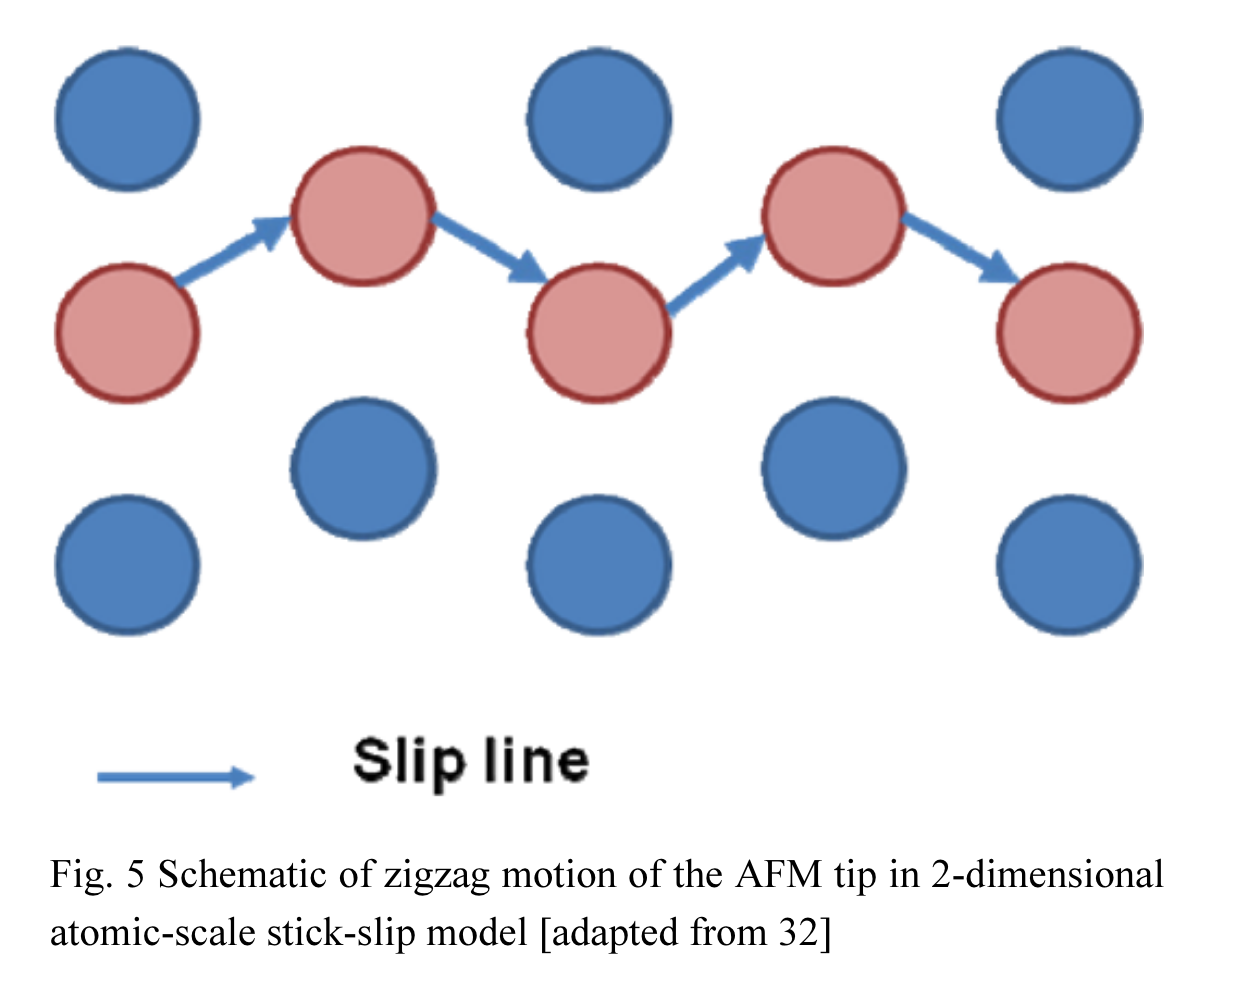
\includegraphics[width=0.5\linewidth]{figures/theory/slip_line.png}
%   \caption{\hl{Temporary} figure from \cite{kim_nano-scale_2009}[p. 144]}
%   \label{fig:slip_line}
% \end{figure}

% \begin{enumerate}
%   \item Friction should decrease by increasing temperature.
%   \item We expect stick slip motion
%   \item What about dependence on normal force?
%   \item Dependence on contact area?
%   \item Dependense on speed? 
% \end{enumerate}

% \begin{itemize}
%   \item Different friction models on macro-and microscopic scale
% \end{itemize}


% Smooth kinetic friction generally increases with speed (velocity strengthening), but sometimes decreases with increasing speed in certain intervals \cite{Manini_2016}.

% the smallest force needed to set a slider in motion – is also dependent on the simulation time (a longer wait may lead to depinning when a short wait might not), and generally dependent on system size, often increasing with sub-linear scaling with the slider’s contact area. To address this kind of behavior in MD simulations, it is often necessary to resort to scaling arguments in order to extrapolate the large-area static friction from small-size MD simulations [131, 140] \cite{Manini_2016}.


% Section 15.3. As shown in Section 15.1, the maximum value of the static friction and the slope of the turning points of the F(x) curves can be used to determine the corrugation U0 of the tip–surface interaction potential and the effective lat- eral stiffness k of the system. From Fig. 18.1(b) we estimate U0 ≈ 0.22 eV and k ≈1N/m. \cite{gnecco_meyer_2015} p. 197






% Concerning stick-slip friction, another problem is that, unlike simulations, real experiments contain mesoscale or macroscale component intrinsically involved in the mechanical instabilities of which stick-slip consists. Here the comforting observation is that stick-slip is nearly independent of speed, so that so long as a simulation is long enough to realize a sufficient number of slip events, the results may already be good enough [148]  \cite{Manini_2016}.


% A serious aspect of stick-slip friction which MD simulation is unable to attack is ageing. The slip is a fast event, well described by MD, but sticking is a long waiting time, during which the frictional contact settles very slowly. The longer the sticking time, the larger the static friction force necessary to cause the slip. Typicall experiments show a logarithmic increase of static friction with time [150] \cite{Manini_2016}.

% Rate and state friction approaches, widely used in geophysics [151], describe phenomenologically frictional ageing, but a quantitative microscopic description is still lacking. Mechanisms invoked to account for contact ageing include chemical strengthening at the interface in nanoscale systems [152], and plastic creep phenomena in macroscopic systems [153]. \cite{Manini_2016}.


% See ``Selected Results of MD Simulations'' in \cite{Manini_2016} p. 24.

% \subsection{Real life experimental procedures}
% From Introduction to Tribology, Second Edition, p. 526: \par The surface force
% apparatus (SFA), the scanning tunneling microscopes (STM), and atomic force and
% friction force microscopes (AFM and FFM) are widely used in nanotribological and
% nanomechanics studies.




\section{Molecular Dynamics}


Maybe read ``Computer Simulations 7 of Nanometer-Scale Indentation
and Friction'' from \cite{BHUSHAN20051507}

Read \cite{Manini_2016}[p. 18]

A promising compromise could possibly be provided by the so-called reactive potentials [120–122], capable of describing some chemical reactions, including interface wear with satisfactory computational efficiency in large-scale atomic simulations, compared to semi-empirical and first-principles approaches. \cite{Manini_2016}




\begin{itemize}
  \item MD simulation (classical or ab initio)
  \item Basics of classical MD simulations: Integration and stuff
  \item Ab initio simulation (quantum mechanics, solving schrödinger)
\end{itemize}



% Quantum-mechanical calculations is more accurate but to numerical intensive.

% Despite recent progress in this respect, it is clear that there will always be
% interesting problems beyond the reach of ab initio approaches
% \cite{PhysRevB.37.6991}.

\subsection{Potentials}
% \cite{PhysRevB.37.6991}

The choices of potentials used in the MD simulation is mainly based on the on
\cite{li_evolving_2016} which have a somewhat similar MD friction simulation,
the difference being that they impose a Si-tip on the graphene sheet supported
by a Si-substrate where we impose drag the whole sheet upon the substrate.
Nonetheless this serves as a good anchor for the methodology of the setup. The
covalent bonds of C-C in graphene and Si-Si in the substrate is described by the
Tersoff and Stillinger–Weber potentials, respectively. A typical 12-6
Lennard–Jones potential is used to describe the van der Waals adhesive
interaction between graphene and the substrate. \\

\subsubsection{General formulation of potentials (?)}

On a general note we can generalize the n-body potential as the expansion in
orders of participating atoms as 
\begin{align*}
  E = \sum_i V_1(\vec{r}_i) + 
      \sum_{\substack{i, j \\ i < j}} V_2(\vec{r}_i, \vec{r}_j) +  
      \sum_{\substack{i,j,k \\ i < j < k}} V_3(\vec{r}_i, \vec{r}_j, \vec{r}_i) + \cdots.
\end{align*} 
where $\vec{r}_n$ is the position of the $n$th particle and $V_m$ is called an
$m$-body potential  \cite{PhysRevB.37.6991}. The first one-body term corresponds
to an external potential, followed by the two-body term, the three-body term and
so on.The simplest model that includes parrticle interaction is the pair
potential truncating the expansion after the two-body term. A general feature of
the pair potentials is that they favor close-packed structures which is unsuited
to describe covalent bonds that take more open structures. In particular, pair
potentials are completely inapplicable to strongly co- valent systems such as
semiconductors \cite{PhysRevB.37.6991}. In order to accomodate the description
of covalent bonds the natural step is thus to include the next step of the
expansion, the three-body terms, as we will see for the modeling of the graphene
sheet C-C bonds and the Silicon sheet Si-Si bonds. For the interaction between
the sheet and the substrate we can nøjes med a Lennard Jones pair potential
describing the non-bonded van der Waals interaction.


\subsubsection{Lennard Jones}
% TODO: Add potential curve figure
This sections is based on [\cite{docs_lammps_LJ}, \cite{C9CP05445F},
\cite{chem_libretexts_LJ}].

The Lennard-Jones (LJ) model is probably one of the most famous pair potentials
used in MD simulations. LJ models the potential energy between two non-bonding
atoms based solely on interatomc distance $r$. The model accounts for attractive
forces arising from dipole-dipole, dipole-induced dipole and London
interactions, and repulsive forces that capture the hard core (is this safe to
say?) of overlapping wave functions at small distances. Thus it is assummes
neutrally charged atoms and was orginally proposed for noble gases. The
classical 12-6 version of the model (refering to the power law of the repulsive
and attractive forces respectively) reads
\begin{align}
  E = 4\epsilon \left[\left(\frac{\sigma}{r}\right)^{12} - \left(\frac{\sigma}{r}\right)^6 \right ], \qquad r < r_c,
  \label{eq:LJ}
\end{align}
where $r$ is the interatomic distance with cut-off $r_c$, $\epsilon$ is the
depth of the potential well and $\sigma$ the distance where the potential is
zero. By solving for the potential minimum ($dE/dr = 0$) we find the equilibrium
distance to be $r_0 = \sigma 2^{1/6}$. This makes for an even cleary
interpration of $\sigma$ which effectively sets the equilirbium distance between
atoms, i.e. the dividing line for which the net force is repulsive or
attractive. While the LJ model in many ways is an oversimplified model that is
insufficient in its description of ... (get source and concrete examples) it is
commonly used as a model for intermaterial interactions (between moving object
and substrate) in friction studies [\cite{li_evolving_2016}, \cite{ZHANG201585},
\cite{kim_nano-scale_2009}].


\subsubsection{Stillinger weber}
% Todo: Add some potential curve figure? or figure of three body angles?
This section is based on [\cite{docs_lammps_sw}, \cite{PhysRevB.31.5262}]

The stillinger weber potential takes the form of a three body potential
\begin{align*}
  E &=\sum_i \sum_{j>i} \phi_2(r_{i j})+\sum_i \sum_{j \neq i} \sum_{k>j} \phi_3(r_{ij}, r_{ik}, \theta_{ijk}),
\end{align*}
where $r_{ij}$ denotes the distance between atom $i$ and $j$ and $\theta_{ijk}$
the angle between bond $ij$ and $jk$. The summations is over all neighbours $j$
and $k$ of atom $i$ within a cut-off distance $r = a\sigma$. \\
The two-body term $\phi_2$ builds from the LJ model with the addition of an
exponetial cutoff term
\begin{align}
  \phi_2(r_{i j}) & =A_{ij} \epsilon_{ij}\left[B_{ij}\left(\frac{\sigma_{ij}}{r_{ij}}\right)^{p_{ij}} - \left(\frac{\sigma_{ij}}{r_{ij}}\right)^{q_{ij}}\right] \exp (\frac{\sigma_{ij}}{r_{ij}-a_{ij} \sigma_{ij}}).
  \label{eq:sw_2}
\end{align}

The model parameters $A$, $\epsilon$, $B$, $\sigma$, $p$, $q$ and $a$ comes with
$i,j$ indices to indicate that theese parameters should be specified for each
unique pair of atom types. However, in our case we will only provide a single
value for each model parameter as we are exclusively dealing with Si-Si bonds.
We see that the first term in eq.~\eqref{eq:sw_2} is reminiscent of the LJ model
in eq.~\eqref{eq:LJ} while the last term effectively drives the potential to
zero at $r=a\sigma$, which is thus the chosen cut-off distance for the potential
evaluation. With the model parameters for the Si-Si modelling (see table
\ref{tab:sw_param}) the cut-off becomes $\sim 3.8$ Å. \\
The three body term includes an angle dependency as
\begin{align}
  \phi_3(r_{ij}, r_{ik}, \theta_{ijk}) &= \lambda_{ijk} \ \epsilon_{ijk} \Big[\cos \theta_{ijk}-\cos \theta_{0,ijk}\Big]^2 \exp (\frac{\gamma_{ij} \sigma_{ij}}{r_{ij} - a_{ij} \sigma_{ij}}) \exp (\frac{\gamma_{ik} \sigma_{ik}}{r_{ik} - a_{ik} \sigma_{ik}}),
  \label{eq:sw_3}
\end{align}
where $\theta_{0,ijk}$ is the equilibrium angle. The first term of
eq.~\eqref{eq:sw_3} includes an angle dependency analog to a harmonic oscillator
based on a cosine angle distance from the equilibrium angle. The final two terms
act again as a cut-off function by driving the potential to zero at $r_{ij} =
a_{ij}\sigma_{ij}$ and $r_{ik} = a_{ik}\sigma_{ik}$ respectively. \\ 
The parameters used for the Si-Si bond modeling is displayed in table
\ref{tab:sw_param} along with an interpretation of each model parameter.



\begin{table}[H]
  \begin{center}
  \caption{Parameters for the stilliner weber potential used for intermolecular interactions in the silicon substrate.}
  \label{tab:sw_param}
  \begin{tabular}{ | c | c | L{9cm} |} \hline
    Parameter & Value & Description \\ \hline 
    $\epsilon$ & 2.1683  & Individual depth of the potential well for each atom
    type pair/tiplets. \\ \hline
    $\sigma$ & 2.0951 & Distance for which the individual pair interactions has
    zero potential (analog to the LJ model). \\ \hline
    $a$ & 1.80 & The individual cut-off distance for each atom type pair. \\
    \hline
    $\lambda$ & 21.0 & The overall depth of the three-body potential well. \\
    \hline
    $\gamma$ & 1.20 & The shape of the three-body cut-off terms. \\ \hline
    $\cos{(\theta_0)}$ & -1/3 & Cosine of equilibrium angle. \\ \hline
    $A$ &  7.049556277 & The overall depth of the two-body potential well. \\
    \hline
    $B$ &  0.6022245584 & Scales the repulsion part of the two-body term. \\
    \hline
    $p$  & 4.0 & The power dependency for the repulsion part of the two-body
    term. \\ \hline
    $q$  & 0.0 & The power dependency for the attraction part of the two-body
    term. \\ \hline
    tol  & 0.0 & LAMMPS: Option to define a different cut-off than the
    theoretical of $r = a\sigma$. $tol = 0$ refers to the theoretical being
    used. \\ \hline
  \end{tabular}
  \end{center}
\end{table}



\subsubsection{Tersoff}
% Add figure similar to:
% https://en.wikipedia.org/wiki/Bond_order_potential#/media/File:Bond-order_interatomic_potential.png,
% showing bond order curves.


% https://interatomic-potentials.readthedocs.io/en/latest/doc/tersoff.html
% https://chem.libretexts.org/Bookshelves/
% Physical_and_Theoretical_Chemistry_Textbook_Maps/Supplemental_Modules_(Physical_and_Theoretical_Chemistry)/Chemical_Bonding/Fundamentals_of_Chemical_Bonding/Bond_Order_and_Lengths
This section is based on [\cite{docs_lammps_tersoff}, \cite{PhysRevB.37.6991}].


The tersoff potential abandon the idea of a general $n$-body form and attempts
instead to build the model on a more physics informed approach; The more
neighbours an atom has the weaker the bonds will be. Thus it introduces the bond
order (bond strentgh), that is environment specific and decrease with increasing
bond coordination (number of neighbours for a given atom). The potential energy
is taken to have the form

\begin{align*}
  E &= \sum_i E_i = \frac{1}{2}\sum_{i \ne j} V_{ij}, \\
  V_{ij} &= f_C(r_{ij}) \big[f_R(r_{ij}) + b_{ij}f_A(r_{ij})  \big],
\end{align*}

% where the total potential energy is decomposed into an atom site energy $E_i$
% and a bond energy $v_{ij}$. 
where the total potential energy is decomposed into a bond energy $V_{ij}$. The
indices $i$ and $j$ run over the atoms of the system with $r_{ij}$ denoting the
distance between atom $i$ and $j$. Notice that the sum includes all combinations
of $i,j$ where $i\ne j$ meaning that the same bond is double counted which is
the reason for the additional factor $1/2$. The reasoning behind comes from the
asymmetry of the bond order $b_{ij}\ne b_{ji}$ leading to a $V_{ij}\ne V_{ji}$.
The bond energy is composed of a repulsive term $f_R$, arising from overlapping
wave functions, and an attractive term $f_A$ associated with bonding. $f_c$ is
simply a smooth cut-off function to increase computational efficiency. $b_{ij}$
represent the bond order, i.e. the strength of the bonds, which depends
inversely on the number of bonds, the bond angles ($\theta_{ijk}$) and
optionally the relative bonds lengths ($r_{ij}$, $r{jk}$). Notice that an
additional cut-off term $a_{ij}$ was orginally multiplied to $f_R$ as a way of
including terms that limit the range of the interactions to the first neighbour
shell. These kind of limitations is already included in $b_{ij}$ for the
attractive term $f_A$ but is often omitted for the repulsive term $f_R$, and we
do so to by setting $a_{ij} = 1$. \\
The cut-off function $f_C$ goes from 1 to 0 over a small interval range $R \pm
D$ as
\begin{align*}
  f_C(r) =
  \begin{cases}
    1 & r < R - D \\
    \frac{1}{2} - \frac{1}{2} \sin{(\frac{\pi}{2} \frac{r - R}{D})} & R - D < r < R + D\\
    0 & r > R + D
  \end{cases},
\end{align*}
which is continuous and differentiable for all $r$. $R$ is usually chosen to
include only the first neighbour shell. \\
The repulsive and attractive terms $f_R$ and $f_A$ is modelled as an exponetial
function, similar to a morse potential, 
\begin{align*}
 f_R(r) &= A \exp(-\lambda_1 r), \\
 f_A(r) &= -B \exp \big(-\lambda_2 r\big).
\end{align*}

The novel feature of the model lies in modeling of the bond order $b_{ij}$ which
includes three-body interactions by summing over a third atom $k \ne i,j$ within
the cut-off $r_{ik} < R + D$ as shown in the following.

\begin{align}
  b_{i j} & =\big(1+\beta^n \zeta_{i j}^n\big)^{-\frac{1}{2 n}} \\
  \zeta_{i j} & =\sum_{k \ne i,j} f_C(r_{i k}) g\Big(\theta_{i j k}\left(r_{i j}, r_{i k}\right)\Big) \exp \left(\lambda_3{ }^m\big(r_{i j}-r_{i k}\right)^m\big) \\
  g(\theta) & =\gamma_{i j k}\left(1+\frac{c^2}{d^2}-\frac{c^2}{\left[d^2+\left(\cos \theta-\cos \theta_0\right)^2\right]}\right).
  \label{eq:tersoff_bond_order}
\end{align}

In eq.~\eqref{eq:tersoff_bond_order} $\zeta_{i,j}$ is an effective coordination
and $g(\theta)$ captures angle dependency as it is minimized at the equilibrium
angle $\theta = \theta_0$. \\
The parameters used to model the graphene C-C bonds is summarized in table
\ref{tab:tersoff_param}



\begin{table}[H]
  \begin{center}
  \caption{Parameters for the tersoff potential used for intermolecular interations in the graphene sheet}
  \label{tab:tersoff_param}
  \begin{tabular}{ | c | c | L{9cm} |} \hline
    Parameter & Value & Description \\ \hline 
    $m$ & 3.0 & Default (not used since $\lambda_3 = 0$ ) \\ \hline
    $\gamma$ & 1.0 & ... \\ \hline
    $\lambda_3$ & 0.0 Å$^{-1}$ & ... \\ \hline
    $c$ & \num{3.8049e4} & Strength of the angular effect \\ \hline
    $d$ & 4.3484 & Determines the ``sharpness'' of the angular dependency \\
    \hline
    $\cos{(\theta_0)}$ & -0.57058 & Cosine of the equilibrium angle \\ \hline
    $n$ & 0.72751 & Power law exponent for the bond order dependency \\ \hline
    $\beta$ & \num{1.5724e-7} & ... \\ \hline
    $\lambda_2$ & 2.2119 Å$^{-1}$ & Decay of repulsion potential term \\ \hline
    $B$ & 346.74 eV & Attractive potential term minimum at core ($ r_{ij} = 0$).
    \\ \hline
    $R$ & 1.95 Å & Center distance for cut-off \\ \hline
    $D$  & 0.15 Å & Thickness of cut-off layers \\ \hline
    $\lambda_1$ & 3.4879 Å$^{-1}$ & Decay of repulsion potential term \\ \hline
    $A$ & 1393.6 eV & Repulsion potential term at core ($ r_{ij} = 0$) \\ \hline
  \end{tabular}
  \end{center}
\end{table}



\subsection{Integration}
% https://www.eng.uc.edu/~beaucag/Classes/AdvancedMaterialsThermodynamics/Books/%5BComputational%20science%20(San%20Diego,%20Calif.)%5D%20Daan%20Frenkel_%20Berend%20Smit%20-%20Understanding%20molecular%20simulation%20_%20from%20algorithms%20to%20applications%20(2002,%20Academic%20Press%20)%20-%20libgen.lc.pdf

Having defined a system of particles governed by interartomic potentials we need
to move the system forward in time. By solving Newtons equations of motion we
effectively do so by sampling the microcanonical ensemble characterized by a
constant number of particles $N$, volume $V$ and energy $E$, hence denoted NVE.
Newtons equaitons of motion read
\begin{align}
  m_i \frac{d^2 \vec{r}_i}{dt^2} = \vec{F}_i = -\nabla U_i
  \label{eq:NE}
\end{align}
where $i$ is the particle index and $m_i$ its mass, $\vec{r}_i = (x_i, y_i,
z_i)$ the position, $t$ is time,  $\nabla_i = (\frac{\partial}{\partial x_i},
\frac{\partial}{\partial y_i}, \frac{\partial}{\partial z_i})$ and $U_i$ the
potential energy. In system the potential energy is a function of the particle
positions of nearby particles depending on the specefic potential in use. Since
the forces defined by the potentials is conservative we expect the energy of the
solution to be conserved. We redefine eq.~\eqref{eq:NE} in terms of two coupled
first order differential equations 
\begin{align}
  \dot{\vec{v}}_i(t) = \frac{\vec{F}}{m_i}, \qquad \dot{\vec{r}}_i(t) = \vec{v}_i(t),
  \label{eq:NE_2}
\end{align}
where $\dot{x} = dx/dt$ (Newton's notation) and $\vec{v} = (v_x, v_y, v_z)$ is
velocity. Numerically we can solve the coupled equations (eq~.\eqref{eq:NE_2}) by
integrating over discrete timnesteps. That is, we discretize the solution into
temporal steps $t_k = t_0 + k\cdot \Delta t$ with time-step $\Delta t$. 

% \begin{align*} \ddot{x}(t) = \frac{F(x)}{m} \quad \rightarrow \quad \dot{x} =
%   v(t), \ \ \dot{v}(t) = \frac{F(x(t))}{m} \end{align*}

% Integration of newtons equations of motion (just like, Euler, Euler cromer and
% so on) and specify the verlet algorithm which is used in Lammps.

% The forces (form the potential) is conservative so the energy should be
% conserved before applying the thermostat.

% However small erros applied by the discrete integraiton algorithm we end up
% having an energy error. This is sensitive to time step. 


\subsubsection{Velocity Verlet}
% http://www.physics.drexel.edu/~valliere/PHYS305/Diff_Eq_Integrators/Verlet_Methods/Diffrntleqn3.pdf
% ttps://www2.ph.ed.ac.uk/~dmarendu/MVP/MVP03.pdf

A common algorithm to integrate Newtons equation of motion (as formulated in
eq.~\eqref{eq:NE_2}) is the \textit{velocity verlet}. We can derive the algorithm
by the use of Taylor expansions. We begin by expanding the next-step position
vector $\vec{r}_i(t + \Delta t)$ at time $t$
\begin{align}
  \vec{r}_i(t + \Delta t) &= \vec{r}_i(t) + \dot{\vec{r}}_i(t) \Delta t + \frac{\ddot{\vec{r}}_i(t)}{2} \Delta t^2 + \mathcal{O}(\Delta t^3) \label{eq:vv_comp1},
\end{align}
where $\ddot{\vec{r}} = d^2\vec{r}/dt^2$ and $\Delta t^n$ is simply the relaxed
notation for $(\Delta t)^n$. Similar we take the expansions of the next-step
velocity vector $\vec{v}_i(t+\Delta t)$ at time $t$ 
\begin{align}
  \vec{v}_i(t+\Delta t) = \vec{v}_i(t) + \dot{\vec{v}}_i(t) \Delta t + \frac{\ddot{\vec{v}}_i(t)}{2}\Delta t^2 + \mathcal{O}(\Delta t^3).
  \label{eq:tay_v1}
\end{align}
Finnally, by taking the expansion of $\dot{\vec{v}}_i(t+\Delta t)$ we can
eliminate the $\ddot{\vec{v}}_i$-term in eq.~\eqref{eq:tay_v1} and simplify it
as shown in the following.
\begin{align}
  \dot{\vec{v}}_i(t+\Delta t) &= \dot{\vec{v}}_i(t) + \ddot{\vec{v}}_i(t) \Delta t + \mathcal{O}(\Delta t^2) \nonumber \\
  \frac{\ddot{\vec{v}}_i(t)}{2}\Delta t^2 &= \frac{\Delta t}{2}\Big( \dot{\vec{v}}(t+\Delta t) - \dot{\vec{v}}_i(t)\Big) + \mathcal{O}(\Delta t^3) \nonumber \\
  &\Downarrow \nonumber \\
  \vec{v}_i(t+\Delta t) &= \vec{v}_i(t) + \dot{\vec{v}}_i(t) \Delta t + \frac{\Delta t}{2}\Big( \dot{\vec{v}}_i(t+\Delta t) - \dot{\vec{v}}_i(t)\Big) + \mathcal{O}(\Delta t^3) \nonumber \\
  &=  \vec{v}_i(t) + \frac{\Delta t}{2}\Big( \dot{\vec{v}}_i(t) +  \dot{\vec{v}}_i(t+\Delta t)\Big) + \mathcal{O}(\Delta t^3).
  \label{eq:vv_comp2}
\end{align}
By combining eq.~\eqref{eq:vv_comp1} and eq.~\eqref{eq:vv_comp2} and using
Newton's second equation $\dot{\vec{v}} = \vec{F}_i(t)/m_i = $ and $\vec{v} =
\dot{\vec{r}}$ we arrive at the final scheme
\begin{align*}
  \vec{r}_i(t + \Delta t) &= \vec{r}_i(t) + \vec{v}_i(t) \Delta t + \frac{\vec{F}_i(t)}{2m_i}\Delta t^2 + \mathcal{O}(\Delta t^3), \\
  \vec{v}_i(t+\Delta t)  &= \vec{v}_i(t) + \frac{\vec{F}_i(t) + \vec{F}_i(t+\Delta t)}{2m_i}  \Delta t + \mathcal{O}(\Delta t^3).
\end{align*}
The scheme will give a local error of order $\Delta t^3$ corresponding to a
global error of $\Delta t^2$. One of the most popular ways to implement this
numerically is as stated in the following steps.
\begin{enumerate}
  \centering
  \item Calculate $v_{k+\frac{1}{2}} = v_k + \frac{F_k}{2m} \Delta t$.
  \item Calculate $r_{k+1} = r_k + v_{k+\frac{1}{2}} \Delta t$.
  \item Evaluate the force $F_{k+1} = F(r_{k+1})$.
  \item Calculate $v_{k+1} = v_{k+\frac{1}{2}} + \frac{F_{k+1}}{2m} \Delta t$  
\end{enumerate}





% \begin{align*} \vec{r}_i(t + \Delta t) &= \vec{r}_i(t) + \vec{v}_i(t) \Delta t
%   + \frac{\vec{F}_i(t)}{2m_i}\Delta t^2 + \mathcal{O}(\Delta t^3), \\
%   \vec{v}_i(t+\Delta t)  &= \vec{v}_i(t) + \frac{\vec{F}_i(t) +
% \vec{F}_i(t+\Delta t)}{2m_i}  \Delta t + \mathcal{O}(\Delta t^3). \end{align*}
% This scheme will give a local error of order $\Delta t^3$ corresponding to a
% global error of $\Delta t^2$. 

% Lets descritize the time as $t_k = k * \Delta t$ with position $\vec{r}_k$ and
% velocity $\vec{v}_k$. At time $t_k$ the acceleration is given $\vec{a}_k =
% F(\vec{r}_k)/m$. We get the implementation steps as follows \begin{enumerate}
% \item Calculate $\vec{r}_{k+1} = \vec{r}_k + \vec{v}_k \Delta t +
% \frac{F(\vec{r}_k)}{2m}(\Delta t)^2$ \item Evaluate $F(\vec{r}_{k+1})$ \item
% Calculate $\vec{v}_{k+1} = \vec{v}_k + \frac{F(\vec{r}_k) +
% F(\vec{r}_{k+1})}{2m} \Delta t$ \end{enumerate}


% It is sometimes expressed as the following. This is mathematically the same,
% but is it computaitonally more efficient?


% \begin{align*} \mathbf{r}_i(t+\delta t) & =\mathbf{r}_i(t)+\mathbf{v}_i(t)
%   \delta t+\frac{\mathbf{f}_i(t)}{2 m_i} \delta t^2 \\
%   \mathbf{v}_i(t+\delta t / 2) & =\mathbf{v}_i(t)+\frac{\delta t}{2}
%   \frac{\mathbf{f}_i(t)}{m_i} \\
%   \mathbf{f}_i(t+\delta t) & =\mathbf{f}_i\left(\mathbf{r}_i(t+\delta
%   t)\right) \\
%   \mathbf{v}_i(t+\delta t) & =\mathbf{v}_i(t+\delta t / 2)+\frac{\delta t}{2}
%   \frac{\mathbf{f}_i(t+\delta t)}{m_i} \end{align*}

%   % https://www2.ph.ed.ac.uk/~dmarendu/MVP/MVP03.pdf Further they suggest this
%   to be the most used algorithm

%   \begin{align*} \mathbf{v}_i(t+\delta t / 2) & =\mathbf{v}_i(t)+\frac{\delta
%     t}{2} \frac{\mathbf{f}_i(t)}{m_i} \\
%     \mathbf{r}_i(t+\delta t) & =\mathbf{r}_i(t)+\mathbf{v}_i(t+\delta t / 2)
%     \delta t \\
%     \vec{f}_i(t + \delta t) &= \vec{f}_i(\vec{r}_i(t+ \delta t)) \\
%     \mathbf{v}_i(t+\delta t) & =\mathbf{v}_i(t+\delta t / 2)+\frac{\delta
%   t}{2} \frac{\mathbf{f}_i(t+\delta t)}{m_i} \end{align*} Make sure to check
%   this out. 

\subsection{Thermostats}

As we already mentioned above in Sec. 2, any kind of sliding friction involves mechanical work, some of which is then transformed into heat (the rest going into structural transformations, wear, etc.). The heat is then transported away by phonons (and electrons in the case of metallic sliders) and eventually dissipated to the environment \cite{Manini_2016}.



Likewise all excitations generated in the simulations should be allowed to propagate in the system and disperese in the bulk of both sheet and substrate. Due to small simulation size theese is likely to relfect back and ´´pile up'' unphysically Thus in order to avoid continuous heating and attain a steady state the (Joule) heat must be removed at a steady state. This is very the viscous damping of the langevin equations enter the picture. It can be difficulut to set the value $\gamma$ for the magnitude of this damping. The unphysical introduction of heat sink can be mittigated by some modifictions he mention, which is kind of next level I guess. 


\subsubsection{Langevin thermostat} \label{sec:langevin}

% Check out \cite{Manini_2016} for a good theory section on this that I had
% completely missed when writing this!

% Based on
% https://www.uio.no/studier/emner/matnat/fys/FYS4130/v19/pensumliste/stat-phys_2019.pdf

% http://physics.gu.se/~frtbm/joomla/media/mydocs/LennartSjogren/kap6.pdf


In order to control the temperature of the system we introduce the so-called
Langevin thermostat. This is a stochastic thermostat that modifies Newtons
equation of motion such that solution lies in the canonical ensemble
characterized by a constant number of particles $N$, constant volume $V$ and
constant temperature $T$, hence denoted NVT. The canonical ensemble system is
represented by the finite system being in contact with an infinte heat bath of
temperature $T$. The NVT ensemble is equivalent to sampling a system in
theromodynamic equilibrium where the weight of each microscopic state is given
by the boltzmann factor $\exp[-E/(k_B T)]$.

The Langevin equation is the modified version of Newtons second law for a
Brownian particle. A brownian particle is a small particle suspendend in liquid,
e.g. pollen or dust, named after Robert brown (1773–1858) who was the first to
observe its jittery motion. The Langevin equation describes this motion as the
combination of viscous drag force $ -\gamma \vec{v}$, where $\gamma$ is a
positive friction coefficient and $\vec{v}$ the velocity vector, and a random
fluctuation force $\vec{R}$. The langevin equation reads
\begin{align}
  m \frac{d \vec{v}}{dt} = -\gamma \vec{v} + \vec{R}
  \label{eq:Langevin}
\end{align}
where $m$ is the particle mass. This effectively describes the particle of
interest, the brownian particle, as being suspendend in a sea of smaller
particles. The collision with these smaller particles is modelled by the drag
force and the fluctuation force. We notice that if the fluctuation force is
excluded eq.~\eqref{eq:Langevin} becomes 
\begin{align*}
  m \frac{d \vec{v}}{dt} = -\gamma \vec{v} \quad \Rightarrow \quad 
  \vec{v}_i(t) = v(0)e^{- \frac{\gamma t}{m}},
\end{align*}
where the solution shows that the brownian particle will come to a complete stop
after a long time ${\vec{v}_i(t\to\infty) \to \vec{0}}$. This is in violation
with the equipartion theorem
\begin{align*}
  \frac{1}{2}m\langle v^2 \rangle_{eq} = \frac{k_B T}{2},
\end{align*}
and hence the fluctuation force is nessecary to obtain the correct equilibrium. 

The following calculations are done in one dimension in order to simplify the
notation. We describe the statistical nature of the collisions as a sum of
independent momentum transfers
\begin{align*}
  \Delta P = \sum_i^N \delta p_i
\end{align*}

where $\Delta P$ denotes the change of momentum after $N$ momentum transfers
$\delta p_i$ from the environment to the brownian particle. We assume the first
and second moments $\langle \delta p \rangle = 0$ and  $\langle \delta p \rangle
= \sigma^2$. When $N$ is large the central limit theorem states that the random
variable $\Delta P$ has a gaussian distribution with  $\langle P \rangle = 0$
and $\langle \Delta P^2 \rangle = N\sigma^2$. If we consider the momentum change
$\Delta P$  over a discrete time $\Delta t$, where the number of collisiosn is
proportional to time $N \propto \Delta t$, the corresponding fluctuation force
$R = \Delta P / \Delta t$ will have a variance 


\begin{align*}
  \langle R^2 \rangle = \frac{\langle \Delta P^2 \rangle}{\Delta t^2} = \frac{N \sigma^2}{\Delta t^2}  \propto \frac{1}{\Delta t}.
\end{align*}

In a computer simulation we need to pick a random force $R(t)$ from a Gaussian
distribution every time-step $\Delta t$. These forces will not be correlated as
long as $\Delta t$ is larger than the correlation time of the forces from the
molecules which we will assume for this model (I think there exist corrections
for this to refer to here). With this assumption we can write the correlation
function as 
\begin{align}
  \langle R(t) R(0) \rangle = 
  \begin{cases}
    \frac{a}{\Delta t}, & |\Delta t| < \Delta t/2 \\
    0, & |\Delta t| > \Delta t/2,
    \label{eq:disc_corr}
  \end{cases}
\end{align}

where $a$ is some strength of (...?). In the limit $\Delta t \to 0$ the
correlation function becomes

\begin{align}
  \langle R(t)R(0) \rangle = a \delta(t),
  \label{eq:F_corr}
\end{align}

% Note that the delta function is justified by the fact that the characteristic frequencies of the phonon and electron excitations are much shorter than the hopping rate of the tip between the minima of the interaction potential \cite{gnecco_meyer_2015}

where $\delta$ denotes the dirac delta function. This is valid for all spatial
coordinates which will all be independent of each other. Since both the drag
force and the fluctuation force originate from the molecular fluid, where the
drag force $-\alpha \vec{v}$ is velocity dependent it is reasonible to assume
that fluctuation force is independent of velocity, i.e. $\langle R_i v_j \rangle
= 0$ for all cartesian indices $i$ and $j$.


% Since $\langle \tilde{F} \rangle = 0$ the random force (fluctuating force)
% will not conribute with a average decay (change) to the velocity. The
% macroscopic decay comes from the friction force (dissipitative force)  $-ma
% =\alpha v$ (give variable explanation). 

In the following we will attempt justify the Langevin equaiton (why it is like
it is) and determine the relationship between the drag coefficient $\gamma$ and
the random force $R$.


From the Langevin equation eq.~\eqref{eq:Langevin} we can compute the velocity
autocorrelation function (Move to appendix?). We do this in one dimension for
simplicity. We begin by multiplying by $(e^{\gamma t /m})/m$

\begin{align*}
  \dot{ v}(t)e^{\gamma t /m} + \frac{\gamma}{m} v(t)e^{\frac{\gamma t}{m}}  = \frac{ F}{m}e^{\frac{\gamma t}{m}},
\end{align*}
and integrate from $t = -\infty$. By the use of integration by parts on the
latter term on the left hand side we calculate the velocity 
\begin{align*}
  \int_{-\infty}^t dt' \ \dot{ v}(t')e^{\frac{\gamma t'}{m}} + \frac{\gamma}{m} v(t)e^{\frac{\gamma t'}{m}} &=  \int_{-\infty}^t dt' \ e^{\frac{\gamma t'}{m}} \frac{ F(t')}{m}  \\
  \int_{-\infty}^t dt' \ \dot{ v}(t')e^{\frac{\gamma t'}{m}} + \left(\Big[ v(t')e^{\frac{\gamma t'}{m}}\Big]_{-\infty}^t - \int_{-\infty}^t dt' \ \dot{ v}(t')e^{\frac{\gamma t'}{m}}\right) &= \int_{-\infty}^t dt' \ e^{\frac{\gamma t'}{m}} \frac{ F(t')}{m}  \\
   v(t) &= \int_{-\infty}^t dt' \ e^{\frac{-\gamma(t - t')}{m}} \frac{ F(t')}{m},
\end{align*}
where $e^{\frac{-\gamma t}{m}}$ plays the role of a response function. We can
then calculate the autocorrelation 
\begin{align*}
  \big\langle  v(t) v(0) \big\rangle &= \int_{-\infty}^t dt_1 \ \int_{-\infty}^0 dt_2 \ e^{\frac{t - t_1 - t_2}{m}} \frac{\langle  F(t_1)  F(t_2) \rangle}{m^2} \\
  &= \int_{-\infty}^t dt_1 \ \int_{-\infty}^0 dt_2 \ e^{\frac{t - t_1 - t_2}{m}} \frac{a \delta(t_1 - t_2)}{m^2} \\
  &= \int_{-\infty}^0 dt_2 \ e^{\frac{t - 2t_2}{m}} \frac{a}{m^2} = \frac{a}{2m\gamma}e^{-\frac{\gamma t}{m}},
\end{align*}
where we used eq.~\eqref{eq:F_corr} and the fact that the integration commutes
with the average (we are allowed to flip the order). By comparing this with the
equipartition theorem we get 
\begin{align*}
  \frac{1}{2}m\langle  v^2 \rangle &= \frac{k_BT}{2} \\
  \frac{1}{2}m\langle  v(0) v(0) \rangle = \frac{a}{4\gamma} &= \frac{k_BT}{2} \\
  a &=  2\gamma k_B T \\
\end{align*}
We notice the appereance of $\gamma$ meaning that the magnitude of the
fluctuations increase both with friction and temperature. Further we can
integrate the velocity over time to get displacement $x(t)$ and show that the
variance (show this? In appendix maybe?) is 
\begin{align*}
  \big\langle x^2(t) \big\rangle = \frac{2 k_B T}{\gamma} \left(t - \frac{m}{\gamma}\left(1 - e^{-\gamma t/m} \right) \right),
\end{align*}
where for $t \gg m/\gamma$ only the $t$-term survies yielding
\begin{align*}
  \langle x^2(t) \rangle = 2 k_BTt/\gamma.
\end{align*}
In 1D, the diffusion constant $D$ is related to the variance as $\langle x^2
\rangle = 2Dt$, meaning that this represents the einstein relation $D = \mu k_B
T$ with the mobility $\mu = 1/\gamma$.

when $t \ll m/\gamma$ we use the Taylor expansion $1 - e^{-x} \approx x - x^2/2$
for $x\ll 1$ to get 
\begin{align*}
  \big\langle x^2(t) \big\rangle = \frac{k_B T}{m} t^2
\end{align*}
which exactly mathces the thermal velocity
\begin{align*}
  v_{\text{th}} \frac{\big\langle x^2(t) \big\rangle}{t^2} = \frac{k_B T}{m}
\end{align*}
which follows from the equipartition theorem. The finite correlation time
$\gamma/m$ hence describe the crossover from the ballistic regime $\sqrt{\langle
x^2(t) \rangle} \propto t$ to the diffusive regime $\sqrt{\langle x^2(t)
\rangle} \propto \sqrt{t}$.

Introduce the fluctuation-dissipation theorem concept earlier since this is a
motivaiton for the Langeivn equation. 


% Of course, this approach is not rigorous, since the relevant particles
% colliding with each given simulated atom are already all included in the
% conservative and deterministic forces explicitly accounted for by the “force
% field”. The Langevin approach is quite accurate to describe small
% perturbations away from equilibrium, but it may fail quite badly in the
% strongly out-of-equilibrium nonlinear phenomena which are the target of the
% present paper.  \cite{Manini_2016}

\subsubsection{Implementing Langevin}
% https://docs.lammps.org/fix_langevin.html

% https://www2.ph.ed.ac.uk/~dmarendu/MVP/MVP03.pdf

% https://chem.libretexts.org/Bookshelves/Physical_and_Theoretical_Chemistry_Textbook_Maps/Non-Equilibrium_Statistical_Mechanics_(Cao)/01%3A_Stochastic_Processes_and_Brownian_Motion/1.04%3A_The_Langevin_Equation

% \cite{Hunenberger2005}(pp. 115, 120-121) \cite{docs_lammps_langevin}

% Make a note: We only introduce the thermostat to the edges of the parts of
% interest as the thermostat might disrupt important properties of the
% simulation (accoridng to Henrik, get a source/example on this).


The implementation of the Langevin equation into LAMMPS follows
\cite{PhysRevB.17.1302} and updates the force vector for each particle as 

\begin{align}
  \vec{F} &= \vec{F_c} + \vec{F}_{f} + \vec{F}_{r} \nonumber \\
  &= -\nabla U - \gamma m \vec{v} + \sqrt{\frac{2 k_B T m \gamma}{\Delta t}}\vec{h}(t)
  \label{eq:Langevin_generalized}
\end{align}
where $\vec{F_c}$ is the conservative force computed via the usual
inter-particle interactions described by the potential $U$, $\vec{F}_f$ is the
drag force and $\vec{F}_r$ is the random fluctuation force where $\vec{h}$ is a
random vector drawn from a normal distribution with zero mean and unit variance.
Notice that this generalized description of the Langevin equation deviates from
the presentation in eq.~\eqref{eq:Langevin} since we have added the conservative
force $\vec{F_c}$, but also by the appearance of the mass in both the drag force
and the fluctuation force due to the introduction of damping. It is beyond out
scope to comprehend this. However, the fact that $\Delta t$ now appears in the
denomiator for the random force variance $2k_B T m \gamma / \Delta t$ is due to
the fact that we have discretized time. This in agreement with the formulation
in eq.~\eqref{eq:disc_corr}. By applying eq.~\eqref{eq:Langevin_generalized} we
get the refined velocity verlet scheme


\begin{align*}
  \vec{v}_i(t + \Delta t/2)  &= \vec{v}_i(t) - \frac{\Delta t}{2}\left(\frac{\nabla_i U(t)}{m_i} + \gamma \vec{v}_i \right) + \sqrt{\frac{k_B T \gamma \Delta t}{2m_i}} \vec{h}_i \\ 
  \vec{r}_i(t + \Delta t) &= \vec{r}_i(t) + \vec{v}_i(t + \Delta t/2) \Delta t \\
  \vec{v}_i(t + \Delta t) &= \vec{v}_i(t+ \Delta t/2) - \frac{\Delta t}{2}\left(\frac{\nabla_i U(t + \Delta t)}{m_i} + \gamma \vec{v}_i(t + \Delta t/2) \right) + \sqrt{\frac{k_B T \gamma \Delta t}{2m_i}} \vec{h}_i
\end{align*}
% A little unsure whether the factor 2 in the denominator in the random force is
% correct.
with new random vector $\vec{h}_i$ for each particle and each update. Notice
however, that LAMMPS only apply this scheme to the particle groups with the
thermostat on. 

% \newpage

% \begin{align} \vec{F}_i &= \vec{f}_{i} + \vec{f}_{f,i} + \vec{f}_{r,i}
%   \nonumber \\
%   m_i \ddot{\vec{r}}_i &= \vec{f}_{i} - \gamma_i \vec{p}_i + \vec{R}_i(t)
%   \label{eq:langevin_old} \end{align}

% where $m_i$ is the mass of particle $i$ $\vec{r}_i$ the position vector. The
% random force $\vec{R}_i(t)$ is described as gaussian white noise and have the
% following properties. 

% \begin{enumerate} \item It is uncorrelated with the velocities
%   $\dot{\vec{r}}(t)$ and deterministic forces $\vec{f}_i(t')$ at previous
%   times $t' < t$. \item The time average is zero: $\langle \vec{R}(t) \rangle
%   = \vec{0}$. \item The mean-square components evaluate to $2m_i\gamma_i k_B
%   T$. \item The force component of particle $i$ $R_{i,\mu}$ along cartesian
%   axis $\mu$ is uncorrelated with any component of particle $j$ $R_{i,\nu}$
%   along cartesian axis $\nu$, unless $i=j$, $\mu=\nu$ and $t=t'$.
%   \end{enumerate}

% The ladder two conditions can be formulated as

% \begin{align*} \langle R_{i,\mu}(t) R_{j,\nu}(t') \rangle = 2m_i \gamma_i k_B
%   T  \delta_{ij} \delta_{\mu\nu}\delta(t'-t),  
% \end{align*}

% where $\delta_{\cdot\cdot}$ is the Kronecker Delta function and
% $\delta(\cdot)$ is the Dirac Delta function. It can be shown that a trajectory
% generated by integrating the Langevin equations of motion
% (eq.~\eqref{eq:langevin_old}) maps a cononical distribution of microstates at
% temperature $T$. \cite{Hunenberger2005}(p.121). (Can I say something more
% about the relationship between the friction froce and the random force - How
% to the balance to give NVT. Is the proof complicated?)\\

% In practice the implementation of the thermostat is implemented discretely by
% updating the force on each particle by the addition of the described forces
% $f_f$ and $f_r$ for each particle. In LAMMPS this is controlled by the user
% defined damping factor ``damp'' = $\gamma^{-1}$ in units of time whih control
% how fast we are going to reach the temperature equlibrium. Thus the
% documentation (\cite{docs_lammps_langevin}) defines the added forces as

% \begin{align*} f_f &= -\frac{m}{\text{damp}}, \qquad f_r \propto \sqrt{\frac{m
%   k_B T}{dt \ \text{damp}}} \end{align*}

% where $v = \dot[r]$ is the velocity. The definition of $f_f$ falls straight
% out of the definition above in eq.~\eqref{eq:Langevin} while the
% proportionality of $f_r$ comes from

% \begin{align*} \sqrt{\langle R(t)^2 \rangle} = \sqrt{2m\gamma k_B T} \propto
%   \sqrt{\frac{m k_B T}{\text{damp}}} \end{align*}

% Thus we have $f_r \propto \sqrt{\langle R(t)^2 \rangle / dt}$ which I do not
% quite understand. It is mentioned in
% \url{https://pubs.acs.org/doi/full/10.1021/ct8002173} when talkikng about
% residual forces, as it is natural when taking a step length of $dt$...
% Probably simply, but check this later. 


% https://www2.ph.ed.ac.uk/~dmarendu/MVP/MVP03.pdf



% \begin{align*} \vec{r}_i(t + \Delta t) &= \vec{r}_i(t) + \vec{v}_i(t) \Delta t
%   + \frac{\vec{F}_i(t)}{2m_i}\Delta t^2 + \mathcal{O}(\Delta t^3), \\
%   \vec{v}_i(t+\Delta t)  &= \vec{v}_i(t) + \frac{\vec{F}_i(t) +
% \vec{F}_i(t+\Delta t)}{2m_i}  \Delta t + \mathcal{O}(\Delta t^3). \end{align*}



% \newpage This section is based on \cite{PhysRevB.17.1302},
% \cite{Hunenberger2005}(pp. 115, 120-121) and \cite{docs_lammps_langevin}



% %
% https://www.uio.no/studier/emner/matnat/fys/FYS4130/v19/pensumliste/stat-phys_2019.pdf

% ``The Langevin equation is Newtons second law for a Brownian particle, where
% the forces include both the viscous drag due to the surrounding fluid and the
% fluctuations caused by the individual collisions with the fluid molecules.''


% % http://physics.gu.se/~frtbm/joomla/media/mydocs/LennartSjogren/kap6.pdf

% % https://www2.ph.ed.ac.uk/~dmarendu/MVP/MVP03.pdf ``Another option to
% simulate a system in the NVT ensemble is to use a stochastic thermostat, as
% opposed to the deterministic thermostat defined through the Nose-Hoover
% equations.''

% ``The equations of mo- tion of a system with a stochastic thermostat are known
% as Brownian dynamic equations''

% In order to simulate the canonical ensemble, that is the ensemble defined by a
% constant amount of particles $N$, constant temperature $T$ and constant volume
% $V$, hence often denoted $NVT$, we apply a so-called thermostat. There exist a
% variety of such including Nosé-Hoover, Gaussian, Berendsen, Langevin
% thermostat and many other (give example of how they modify) We will use the
% ladder. \\
% The connical ensemble is an ensemble of systems by the assumption that the
% system of interests is connected to an infitely large heat bath of temperature
% $T$. The Langevin thermostat assumes that the particles collides with much
% smaller lighter particles representing the heat bath as a sea of small
% particles. The collisions is described by a friction force $f_f = -\gamma
% \vec{p}$, where $\gamma$ is positiv friction coefficient and $\vec{p}$ the
% momentum vector, and a random force $f_r = \vec{R}_i(t)$. By denoting the
% conservative force arising from the usual inter-particle interactions
% $\vec{f}_i$ on particle $i$ we get the Langevin equations of motion describing
% the total force $\vec{F}_i$ on particle $i$ as

% see https://www2.ph.ed.ac.uk/~dmarendu/MVP/MVP03.pdf p. 4


\subsection{MD limitations (?)}

% One of the limitations of concern is in regard to the simulation scale. Despite relatively fast processor speed and efficient algorithm the number of atoms that can be handled realistically is still insufficient for complex system simulation \cite{kim_nano-scale_2009}.



% The main problem when studying the velocity dependence of friction by MD
% simulations is the fact that speeds below few m/s are not accessible. These
% values are well above typical speeds at which atomic stick–slip is resolved by
% AFM (nm/s to μm/s). The reason for that is the typical time scales in MD, which
% are of the order of 1 fs. Furthermore, phenomena such as thermally activated
% hopping are not effective at high speeds, which makes any attempts to
% extrapolate the model predictions on the velocity dependence of friction quite
% doubtful. A possible solu- tion consists of accelerating the simulations during
% the long stick phases separating rapid slip events. \cite[p.
% 207]{gnecco_meyer_2015}


\subsection{LAMMPS}


\section{Defining the system}

The simmulated system consist of two major parts: A 2D graphene sheet and a 3D Silicon ``bulk'' substrate. These parts interact with a van der Waals force (modelled by the LJ potential). We apply a normal load to the sheet inducing a normal force response between the sheet and substrate. By dragging the sheet along the substrate we measure the responding frictional forces.


\subsection{Region definitions (Sheet, pullblocks and substrate)}

The system, sheet and substrate, is further subdivided according to
functionality in the MD simmulations. The sheet ends is reserved for so-called
\textit{pull blocks}, which is used application of normal load, stretching and
dragging the sheet, and as a thermostat, while the remaining \textit{inner
sheet} is left as an untouched (NVE) canvas for kirigami cuts. The pull blocks
are equal split between a thermostat part and a rigid part which is locked into
a single rigid body after an initial relaxtion period. Note that the rigid part
of the pull blocks on both side is considered a single rigid object even though
they are physically seperated. This means that all force interactions on these
parts will be applied as a common average making the move in total
synchronization. The substrate is equally divided into three parts: The
\textit{upper layers} (NVE) responsible for the sheet-substrate interaction, the
\textit{middle layers} being a thermostat (NVT), and the \textit{bottom layers}
is frozen (rigid and fixed) in the initial lattice structure to ensure that the
substrate stays in place. In figure \ref{fig:system} the system is displayed
with colors matching the three distinct roles:
\begin{enumerate}
  \item Red: NVE parts which is governing the frictional behaviour of interest.
  \item Green: Thermostats (NVT) sourrounding the NVE parts in order to modify the temperature without making disturbing changes to the interaction of the sheet and substrate.
  \item Blue: Parts that is initially or eventually turned in to rigid objects. For the substrate this is additionally locked off and immobile. 
\end{enumerate}

The total system size in terms of atom count is given in table \ref{tab:system_count} while the sheet length dimension is given in table \ref{tab}

The total system size (without cuts in the sheet) is 27456 atoms, and the distribution into the various regions is shown in table \ref{tab:system_count}. The length dimensions of the sheet is given in table \ref{tab:sheet_dim}.

\begin{figure}[H]
  \centering
  \begin{subfigure}[b]{0.80\textwidth}
      \centering
      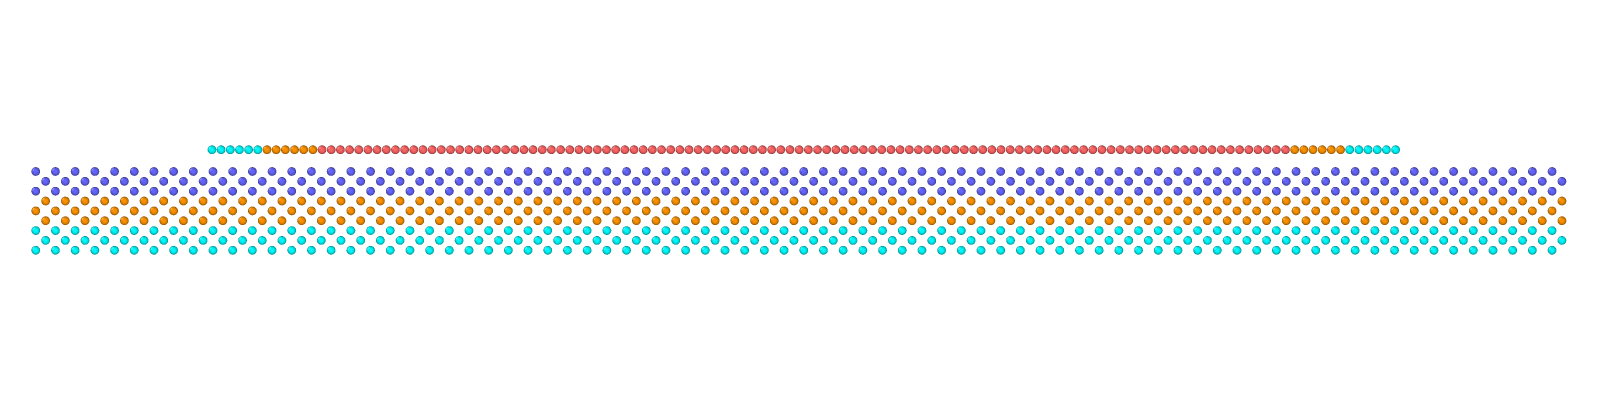
\includegraphics[width=\textwidth]{figures/system_sideview.png}
      \caption{Side view showing sheet on top of the substrate.}
      \label{fig:sideview}
  \end{subfigure}
  \hfill
  \begin{subfigure}[b]{0.80\textwidth}
      \centering
      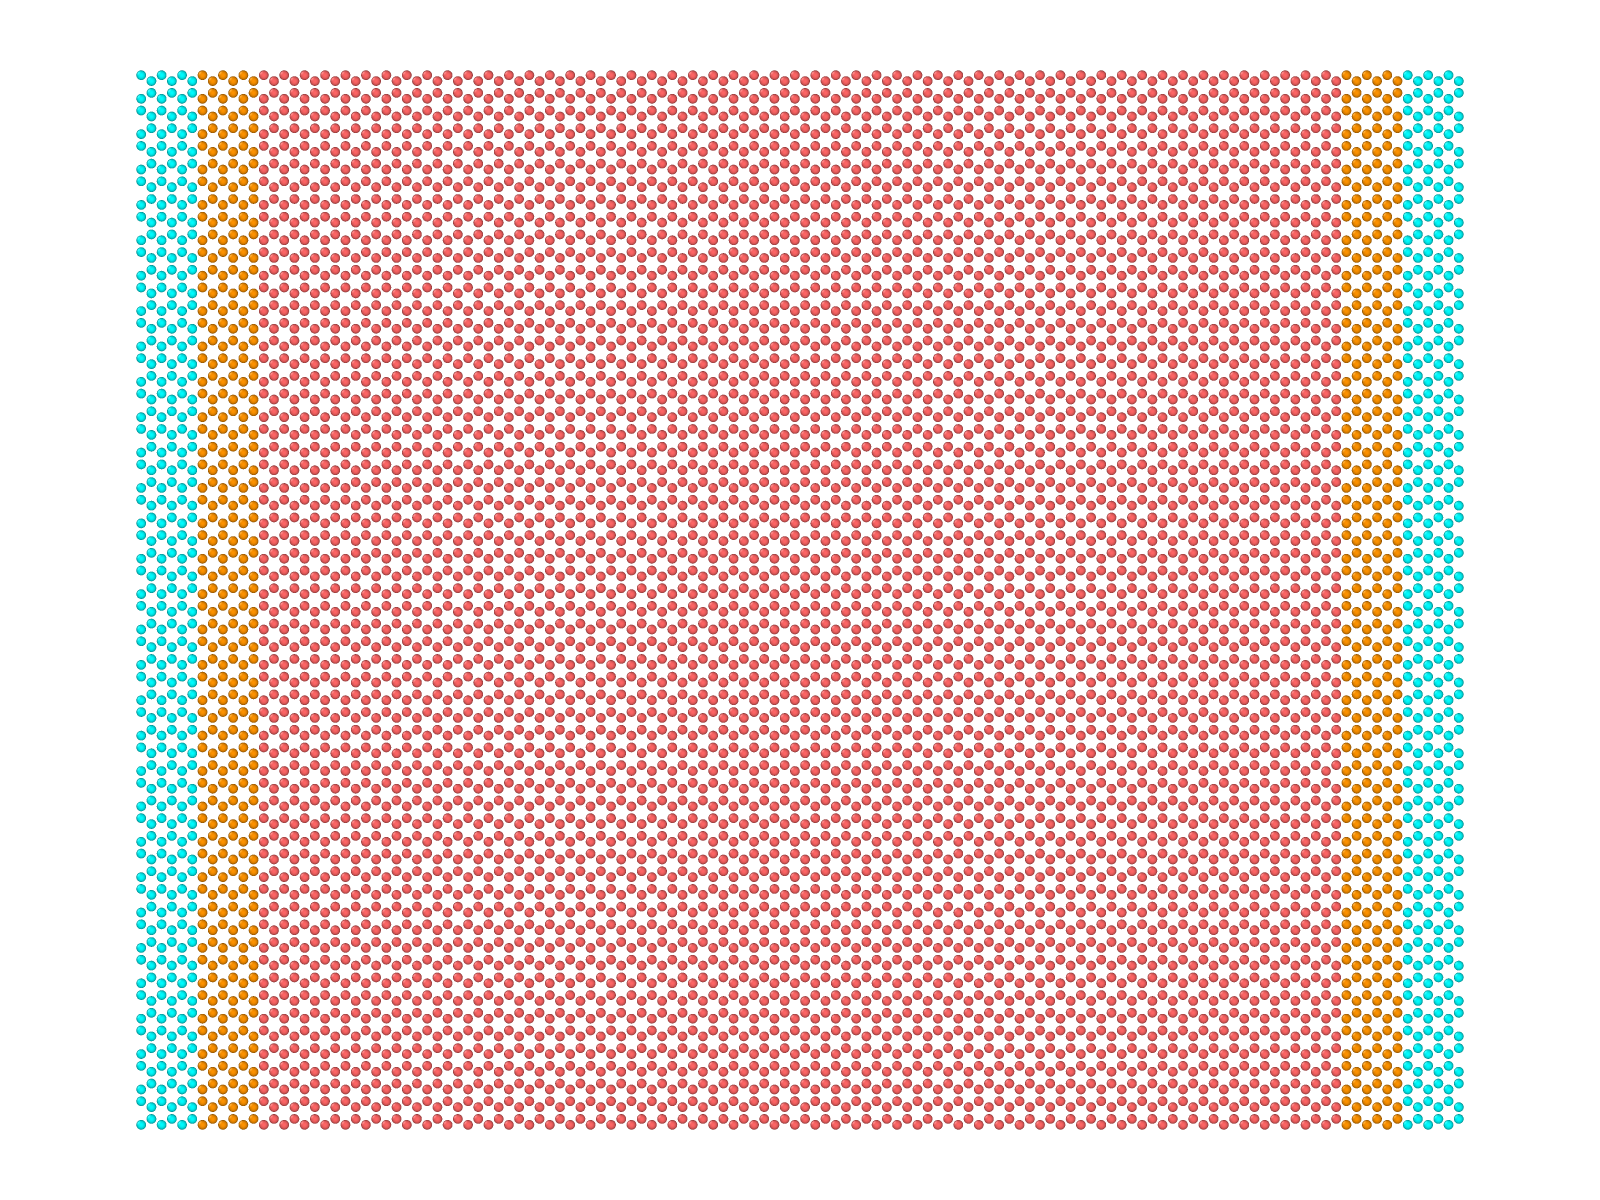
\includegraphics[width=\textwidth]{figures/system_topview.png}
      \caption{Top view showing only the sheet.}
      \label{fig:topview}
  \end{subfigure}
  \hfill
     \caption{System configuration colorized to indicate NVE parts (red), thermostat parts (green) and rigid parts (blue).}
     \label{fig:system}
\end{figure}

\begin{table}[H]
  \begin{center}
  \caption{Amount of atoms in the various system regions in the case of no cutting applied to the sheet.}
  \label{tab:system_count}
  \begin{tabular}{ |c|| c | c | c | c | c | c |} \hline
    \textbf{Region} & \textbf{Total}  & Sub region & Sub total & \textbf{NVE} &
    \textbf{NVT} & \textbf{Rigid} \\ \hline   
    \multirow{2}{*}{Sheet} & \multirow{2}{*}{7800} & Inner sheet & 6360 & 6360 &
    0 & 0 \\ %\hline
    & & Pull blocks & 1440 & 0 & 720 & 720 \\ \hline   
    \multirow{2}{*}{Substrate} & \multirow{2}{*}{19656} & Upper & 6552 & 6552 &
    0 & 0 \\ %\hline
    & & Middle & 6552 & 0 & 6552 & 0 \\ %\hline
    & & Bottom & 6552 & 0 & 0 & 6552 \\ \hline \hline   
    All & 27456 & \multicolumn{2}{r|}{} & 12912 & 7272 & 7272 \\ \hline 
  \end{tabular}
  \end{center}
\end{table}


\begin{table}[H]
  \begin{center}
  \caption{Sheet dimensions comparing the full sheet to its subdivisions: inner sheet and pull blocks.}
  \label{tab:sheet_dim}
  \begin{tabular}{ | l | r@{}l | r@{}l | c |} \hline
    \textbf{Group} & \multicolumn{2}{c|}{$x,y$-dim} & \multicolumn{2}{c|}{dim
    [Å]} & Area [Å$^2$]\\ \hline
  Full sheet & $x_S \: \times \: $ & $y_S$ &  $130.029 \: \times \:$ & $163.219$
  Å & $\phantom{2\times} 21,223.203$ \\ \hline
  Inner sheet & $x_S \: \times \:$ & $81.40 \ \%_{y_s}$ &  $130.029  \: \times
  \:$ & $132.853$ Å & $\phantom{2\times} 17,274.743$\\ \hline
  Pull blocks & $2 \times x_S \: \times \:$ & $ \phantom{0}9.30 \ \%_{y_s}$ & $2
  \times 130.029  \: \times \: $ & $\phantom{0}15.183$ Å  & $2 \times
  \phantom{0}1,974.230$ \\ \hline  
  \end{tabular}
  \end{center}
\end{table}


\subsection{Numerical procedure}

The numerical procedure for the friction simulations can be arranged as the following.

\begin{enumerate}
  \item Relax (15 ps): The sheet and substrate is relaxed for 15 ps. They are
  both initially added in their crystaline form. The sheet is constrained under
  three hard spring forces (spring constant $10^5$ eV/Å$^2$ $\sim$ \num{1.6e6} N/m): One spring
  attathes the sheet center of mass (CM) to its orginal postion preventing
  drift, while the remaining two is attatched to the CM for the pull blocks to
  their initial position respectively to prevent rotation. These spring forces
  are immediately terminated after the relax phase. In this phase the pull
  blocks is only rigid with respect to the z-direction (perpendicular to the
  sheet). That is, all the forces in the z-direction is summed up and
  distributed on the pull blocks while it is free to expand and contract in the
  x-y-plane. This is mainly to ensure that is achieves the correct lattive
  spacing according to the temperature of the system. For the remaining phases
  the rigid parts of the pull block is in fact rigid with respect to all
  directions. 
  \item Stretch: The sheet is stretched by seperating to opposing rigid parts of
  the pullblock at constant velocity until the desired stretch amount is met. 
  \item Pause 1 (5 ps): The sheet is relaxed for 5 ps after the stretch
  procedure.
  \item Pause 2 (Normal load): The normal load is applied to the rigid parts of
  the pull blocks together with a damping force to prevent hard impact between
  sheet and substrate as the seperating distance is now reduced depending on the
  strength of the normal load. The damper is terminated after 0.5 ps, as this
  was suitable for the extreme load cases of our force range, and the system is
  relaxed until a total of 5 ps has passed.
  \item Drag: A virtuel atom is introduced into the simulation which exclusively
  interacts with the rigid parts of the pull through a spring force with variable spring constant $K$ in the x-y-plane. The z-direction is not affected by the spring force and is governed by the balance between normal load and the normal force response from the sheet-substrate interaction. The virtual atom is immediately given a constant velocity corresponding to a variable \textit{drag speed} parameter
\end{enumerate}

At the initial timestep the three nearest neighbours (at distance 1.42 Å) of all graphene atoms is recorded. If these nearest neighbours exceed a threshold of 4 Å this is raises a rupture flag which halt the simulation early. Thus, we effectively prevent any kind of wear on the sheet. For the substrate we do not perform such an analysis but only visually confirms that no wear is accouring under the most extreme simulation parameters. 

\subsection{Creating the sheet}

We are going to create a 2D sheet graphene sheet. 

\subsubsection{Graphene}
% (https://community.wvu.edu/~miholcomb/graphene.pdf)
% https://www.physics-in-a-nutshell.com/article/4/lattice-basis-and-crystal

Graphene is a single layer of carbon atom, graphite is the bulk, arranged in a
hexagonallattice structure. We can describe the 2D crystal structure in terms of
its primitive lattice vector and a basis. That is we populate each lattice site
by the given basis and translate it to fill the whole plane by any linear
combination of the lattice vectors
\begin{align*}
  \vec{T}_{mn} = m\vec{a_1} + n\vec{a_2}, \qquad m,n \in \mathbb{N}.
\end{align*}
For graphene we have the primitive lattice vectors 
\begin{align*}
  \vec{a_1} = a \left(\frac{\sqrt{3}}{2}, -\frac{1}{2}\right), \qquad \vec{a_2} = a \left(\frac{\sqrt{3}}{2}, \frac{1}{2}\right), \qquad |\vec{a_1}| = |\vec{a_2} = 2.46 \ \text{Å}.
\end{align*}
Notice that we deliberately excluded the third coordinate as we only consider a
single graphene layer on not the bulk graphite consisting of multiple layers
stacked on top of each other. The basis is 
\begin{align*}
  \Big\{\Big(0,0\Big), \frac{a}{2}\Big(\frac{1}{\sqrt{3}}, 1 \Big) \Big\}
\end{align*}
It turns out that the spacing between atoms is equal for all paris with an
interatomic distance 
\begin{align*}
  \left|\frac{a}{2}\Big(\frac{1}{\sqrt{3}}, 1 \Big)\right| \approx 1.42 \ \text{Å}.
\end{align*}


\begin{figure}[H]
  \centering
  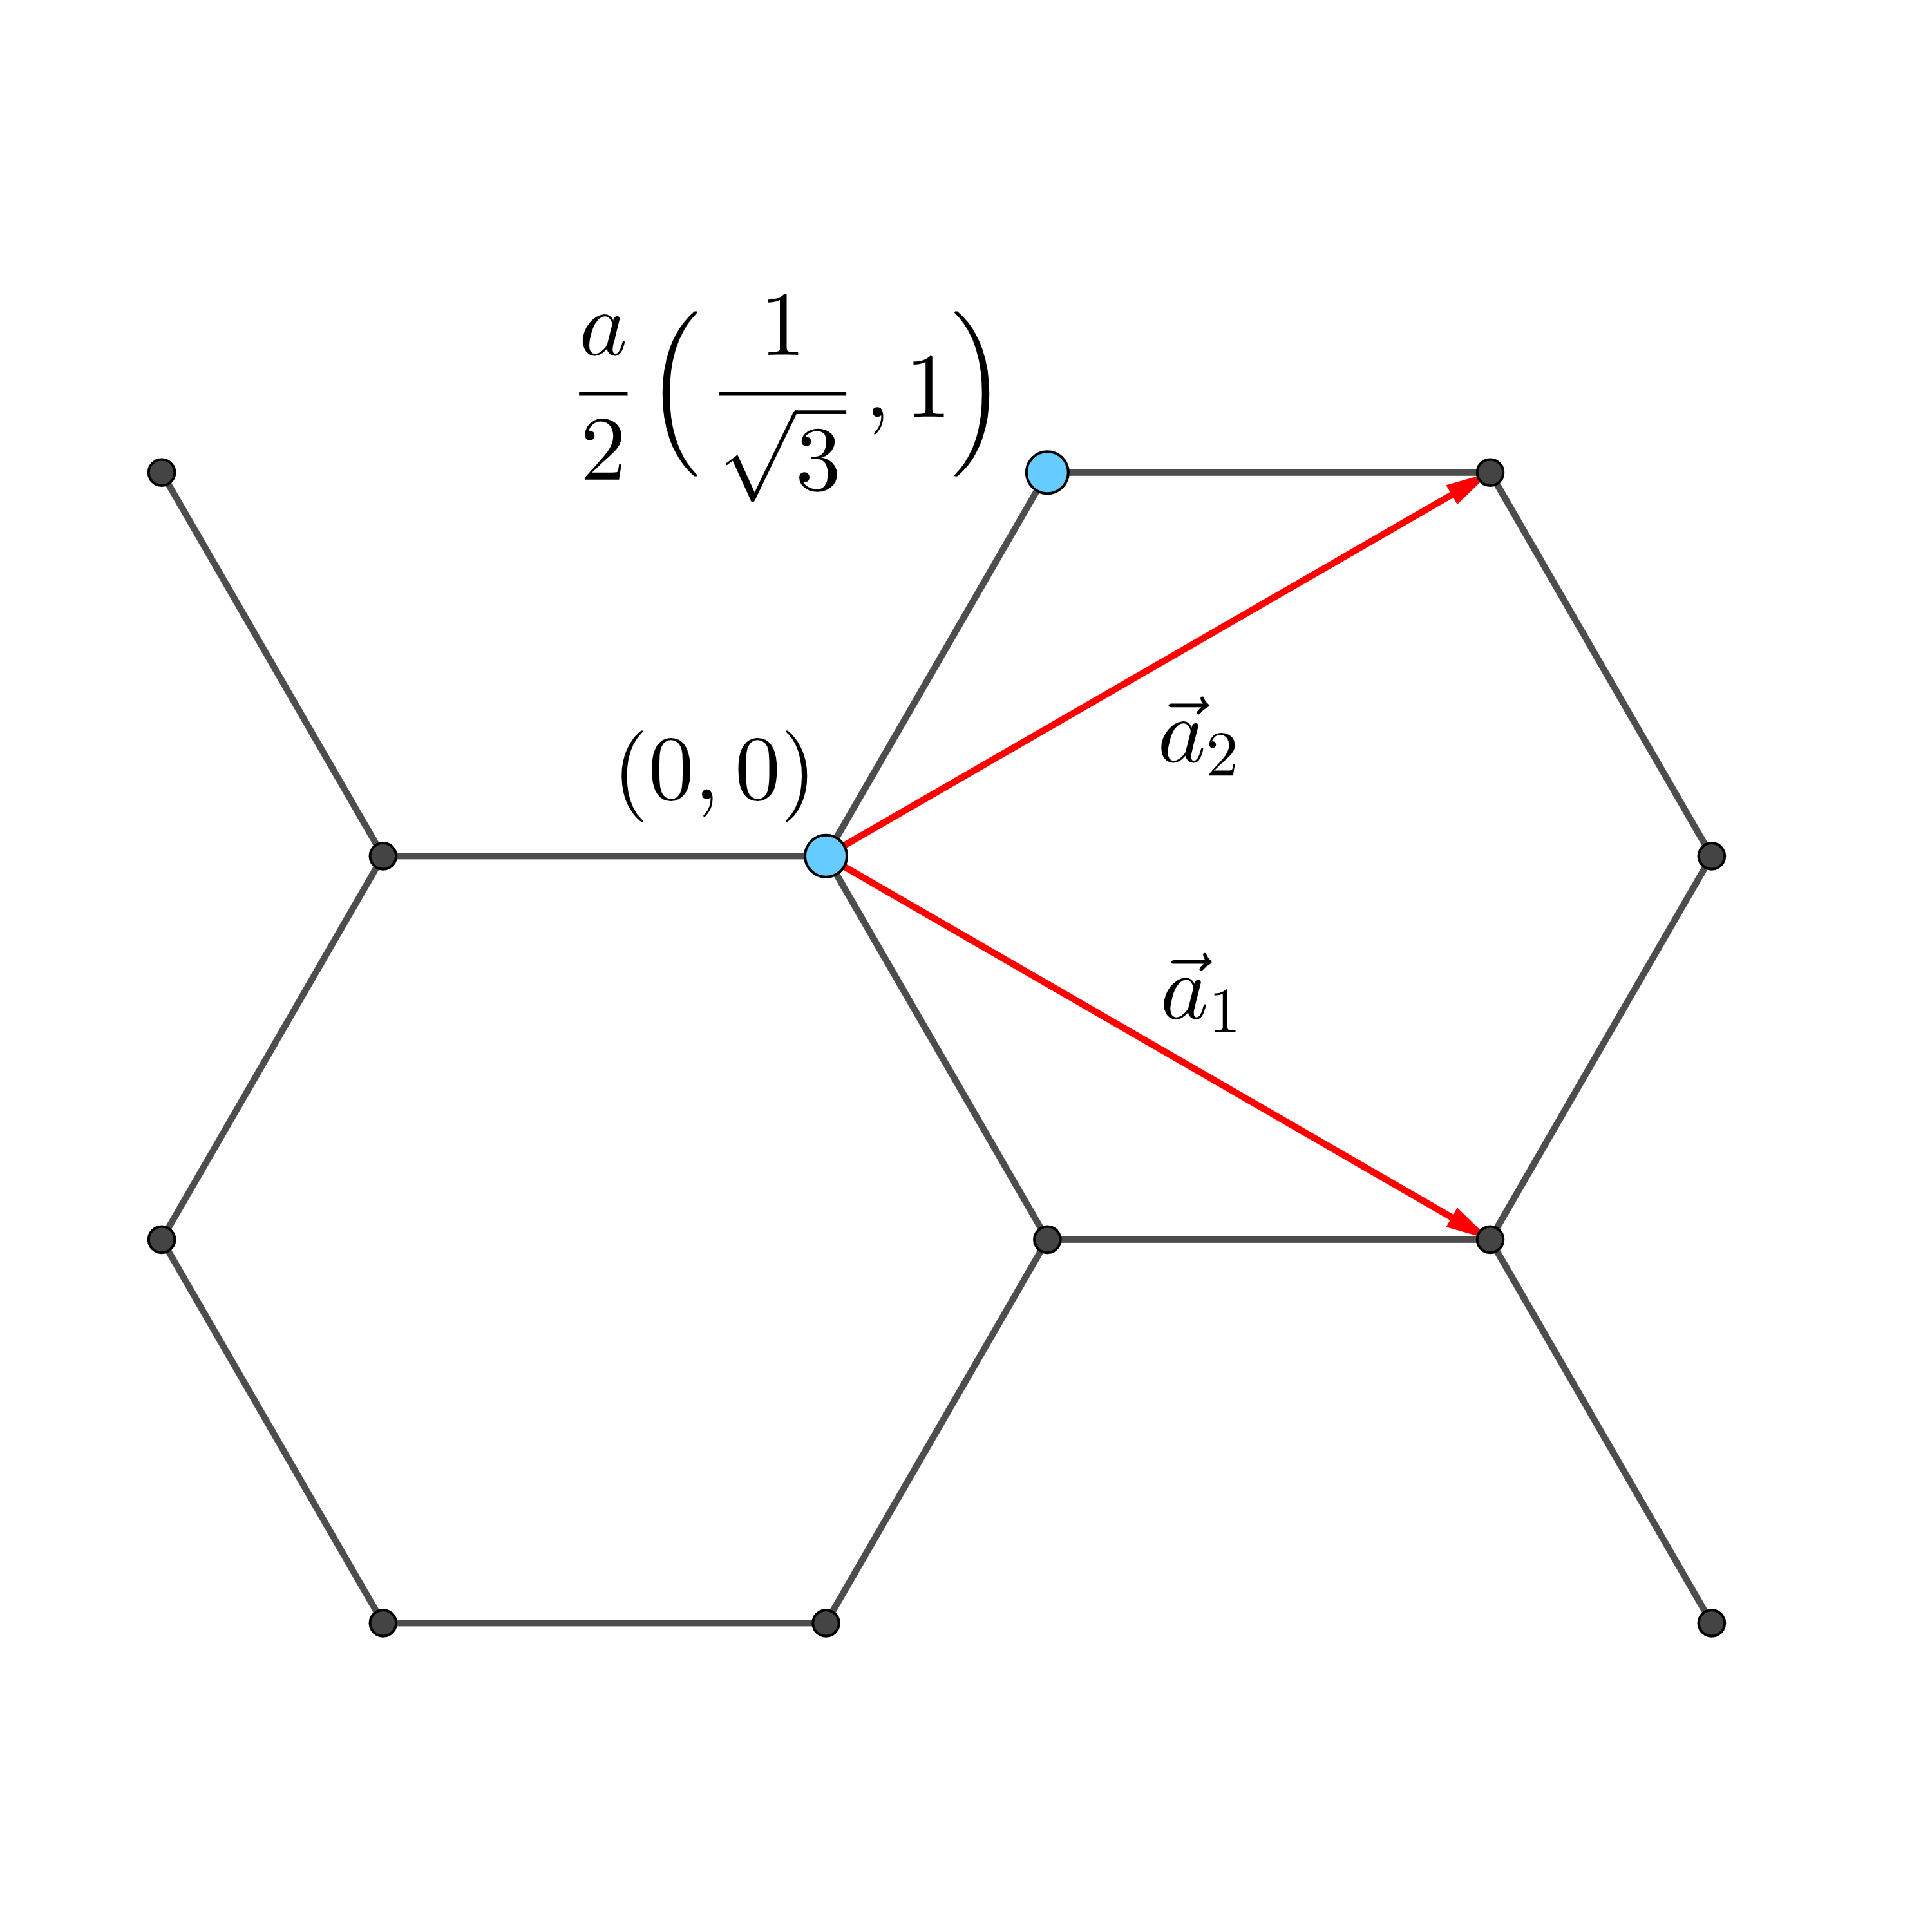
\includegraphics[width=0.3\linewidth]{figures/crystal.png}
  \caption{Graphene crystal structure with basis.}
  \label{fig:graphene_crystal}
\end{figure}



\subsubsection{Indexing}

In order to define the cut patterns applied to the graphene sheet we must define
an indexing system. We must ensure that this gives an unique description of the
atoms as we eventually want to pass a binary matrix, containg 0 for removed atom
and 1 for present atom, that uniquely describes the sheet. We do this by letting
the x-coordinate point to zigzag chains and the y-coordinate to the position
along that chain. This is illustrated in figure \ref{fig:atom_indexing}. Other
solutions might naturally invole the lattice vectors, but as these only can be
used to translate to similar basis atoms a unfortunate duality is introduced as
ones need to include the basis atom of choice into the indexing system. With the
current system we notice that locallity is somewhat preserved. That is, atom
$(i, j)$ is in the proximity of $\{(i+1, j), (i-1, j), (i, j+1), (i, j-1)\}$,
but only three of them is categorized as nearest neighbours due to the hexgonal
structure of the lattice. While $(i, j\pm 1)$ is always nearest neighbours the
neighbour in the x-direction flip sides with incrementing y-coordinate. That is
the nearest neighbours (NN) is decided as
\begin{align*}
  j \ \text{is even} &\rightarrow \text{NN} = \{(i+1, j), (i, j+1), (i, j-1)\}, \\
  j \ \text{is odd} &\rightarrow \text{NN} = \{(i-1, j), (i, j+1), (i, j-1)\}.
\end{align*}

\begin{figure}[H]
  \centering
  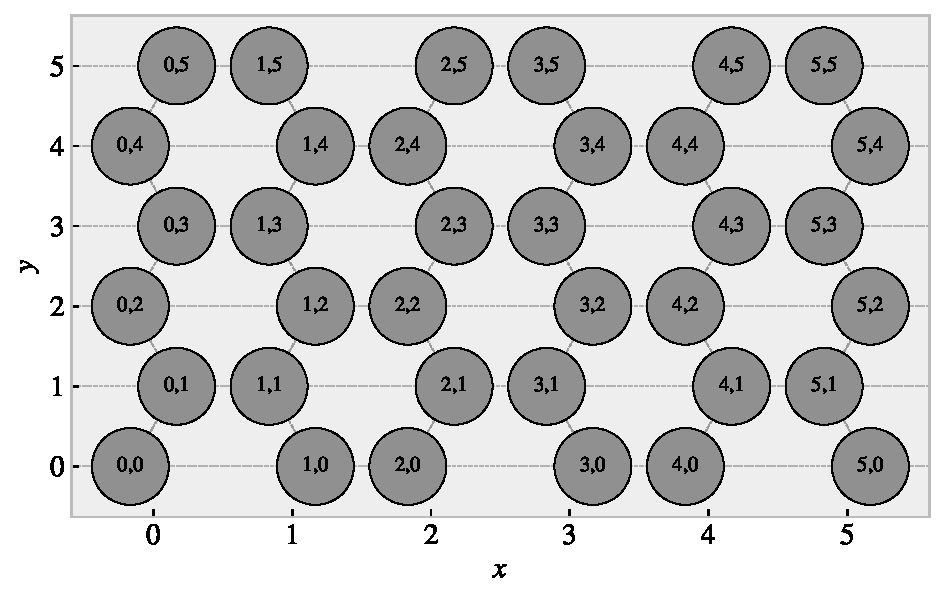
\includegraphics[width=0.7\linewidth]{figures/atom_indexing.pdf}
  \caption{Graphene atom indexing}
  \label{fig:atom_indexing}
\end{figure}

\subsubsection{Removing atoms}

As a mean to ease the formulation of cut patterns we introduce pseudo center
element in each gap of the hexagonal honeycombs, see figure
\ref{fig:center_indexing}. 

\begin{figure}[H]
  \centering
  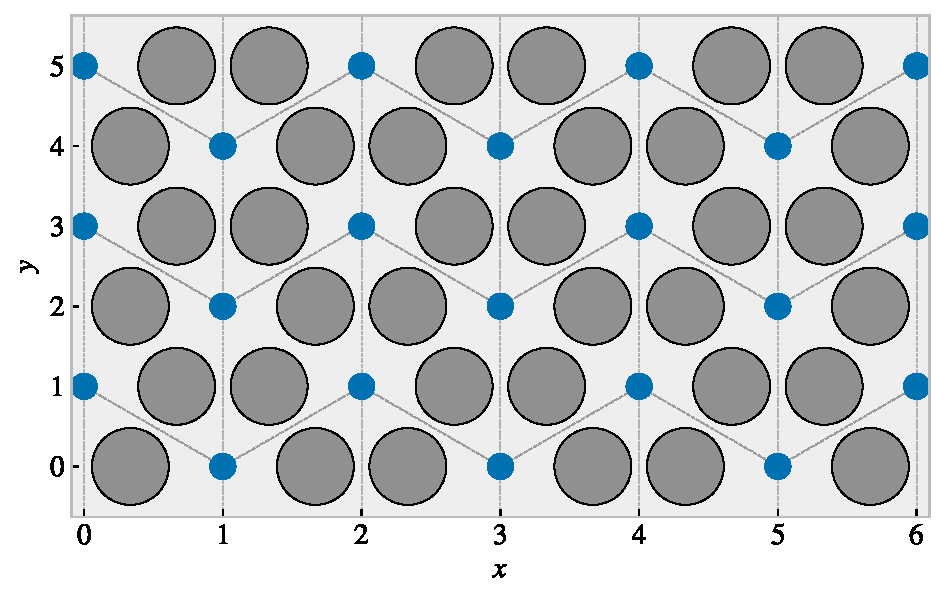
\includegraphics[width=0.7\linewidth]{figures/center_indexing.pdf}
  \caption{Graphene center indexing}
  \label{fig:center_indexing}
\end{figure}




Similar to the case of the indexing for the carbon atoms themself the nearest
neighbour center elements alternate with position, this time along the
x-coordinate. Each center element has six nearest neighbours, in clock wise
direction we can denote them: ``up'', ``upper right'', ``lower right'',
``down'', ``lower left'', ``upper left''. The ``up'' and ``down'' is always
accesed as $(i,j\pm 1)$, but for even $i$ the $(i+1,j)$ index corresponds to the
``lower right'' neighbour while for odd $i$ this corresponds to the ``upper
right'' neighbour. This shifting applies for all left or right neighbours and
the full neighbour list is illustrated in figure \ref{fig:center_directions}. 


\begin{figure}[H]
  \centering
  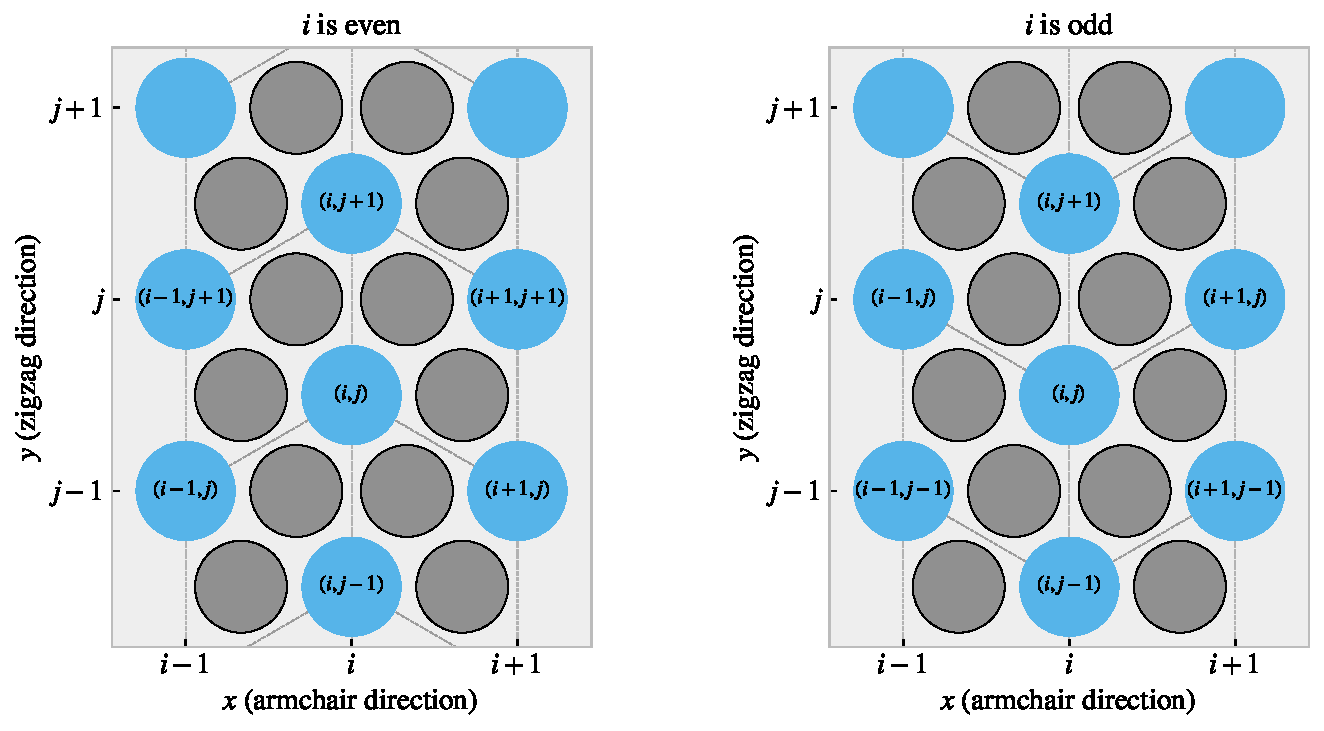
\includegraphics[width=0.7\linewidth]{figures/center_directions.pdf}
  \caption{Graphene center elements directions}
  \label{fig:center_directions}
\end{figure}


We define a cut pattern by connecting center elements into connected paths. As
we walk element to element we remove atoms according to one of two rules 
\begin{enumerate}
  \item Remove intersection atoms: We remove the pair of atoms placed directly
  in the path we are walking. That is, when jumnping to the ``up'' center
  element we remove the two upper atoms located in the local hexagon of atoms.
  This method is sensitive to the order of the center elements in the path. 
  \item Remove all surrounding atoms: We simply remove all atoms in the local
  hexagon surrounding each center element. This method is indepdent of the
  ordering of center elements in the path.
\end{enumerate}

We notice that removing atoms using either of these rules will not garuantee an
unique cut pattern. Rule 1 is the more sensitive to paths but we realize that,
for an even $i$, we will remove the same five atoms following either of the
following paths.
\begin{align*}
  (i, j) &\rightarrow \underbrace{(i+1,j+1)}_{\text{upper right}} \rightarrow \underbrace{(i, j+1)}_{\text{up}} \rightarrow \underbrace{(i+1, j+2)}_{\text{upperright + up}} \rightarrow \underbrace{(i+1, j+1)}_{\text{upper right}} \\
  (i, j) &\rightarrow \underbrace{(i+1,j+1)}_{\text{upper right}} \rightarrow \underbrace{(i+1, j+2)}_{\text{upperright + up}} \rightarrow \underbrace{(i, j+1)}_{\text{up}}
\end{align*}

For rule 2 it is even more abovious that different paths can result in the same
atoms being removed. This is the reason that we needed to define and indexing
system for the atom position itself even though that all cuts generated manually
will use the center element path as reference. \\

Illustrate some delete path?



\subsection{Kirigami patterns}
\subsubsection{Pop-up}
\subsubsection{Honeycomb}
\subsubsection{Random walk}






\section{Fourier Transform (light)}
% https://www.brown.edu/research/labs/mittleman/sites/brown.edu.research.labs.mittleman/files/uploads/lecture21_0.pdf
% https://mathworld.wolfram.com/FourierTransform.html

% https://lpsa.swarthmore.edu/Fourier/Xforms/FXformIntro.html
\textbf{Find out where to put this if nessecary}. \\

Fourier transform is a technique where we transform a function $f(t)$ of time to
a function $F(k)$ of frequency. The Forward Fourier Transform is done as
\begin{align*}
  F(k) = \int_{-\infty}^\infty f(t) e^{-2\pi ikx} dx
\end{align*}

For any complex function $F(k)$ we can decompose it into magnitude $A(k)$ and
phase $\phi(k)$
\begin{align*}
  F(k) = A(k) e^{i \phi(k)}
\end{align*}

Hence when performing a Forward Fourier transform on a time series we can
determine the amplitude and phase as a function of freqeuncy as 
\begin{align*}
  A(k) = |F(k)|^2, \qquad \phi(k) = \Im{\ln{F(k)}}
\end{align*}






\begin{itemize}
  \item Real life procedures to mimic in computation, for instance Atomic Force
  Microscoopy (AFM) for friction measurements.
  \item Available technology for test of my findings if successful
  (possibilities for making the nano machine) 
\end{itemize}


\section{Machine Learning (ML)}
\begin{itemize}
  \item Feed forward fully connected
  \item CNN
  \item GAN (encoder + decoder)
  \item Genetic algorithm
  \item Using machine learning for inverse designs partly eliminate the black
  box problem. When a design is produced we can test it, and if it works we not
  rely on machine learning connections to verify it's relevance. 
  \item However, using explanaitons techniques such as maybe t-SNE, Deep dream,
  LRP, Shapley values and linearizations, we can try to understand why the AI
  chose as it did. This can lead to an increased understanding of each design
  feature. Again this is not dependent on the complex network of the network as
  this can be tested and veriied independently of the network. 
\end{itemize}

\subsection{Feed forward network / Neural networks}
\subsection{CNN for image recognition}
\subsection{GAN (encoder + deoder)}
\subsection{Inverse desing using machine learning}
\subsection{Prediction explanation}
\subsubsection{Shapley}
\subsubsection{Lineariations}
\subsubsection{LRP}
\subsubsection{t-SNE}



